\documentclass[12pt, a4paper]{extarticle}
\usepackage{cmap}
\usepackage{amsfonts}
\usepackage[T2A]{fontenc}
\usepackage[utf8]{inputenc}
%\usepackage{mathtext}  
\usepackage{amsmath, amsfonts, amssymb}
\usepackage[russian]{babel}
\usepackage[body={17.5cm, 23.5cm},left=3cm, top=2cm, right=2cm]{geometry}
\usepackage{graphicx}
\usepackage{blindtext}
\usepackage{fancyhdr}
\usepackage{graphicx}
\usepackage{ragged2e}
\usepackage{epigraph}
\usepackage{misccorr}  
\usepackage{indentfirst} 
\usepackage{amsmath}
\usepackage{tabularx} 

\usepackage{fancyhdr} 
\usepackage{color}

\usepackage{makecell}
\usepackage{slashbox}

\usepackage{enumitem}
\usepackage{float}

%\parindent{1.25cm} 
\graphicspath{images/}
\setcounter{tocdepth}{6}
\newcommand{\eps}{\varepsilon}
\newcommand{\re}{\operatorname{Re}}
\newcommand{\im}{\operatorname{Im}}

\newcommand{\lb}{\textquotedblleft}
\newcommand{\rb}{\textquotedblright}

\DeclareMathOperator{\sgn}{sgn}
\renewcommand{\labelitemi}{$-$}
\renewenvironment{itemize}[1][{---\hfil}]{\begin{list}{#1}{\topsep=0pt\parsep=0pt plus 1pt\itemsep=\parsep\leftmargin=0pt \itemindent=\parindent}\addtolength{\itemindent}{\labelwidth}}{\end{list}}

\numberwithin{equation}{section} 

\newtheorem{attachment}{\hspace{12cm}  Приложение}
\renewcommand{\theattachment}{\Alph{attachment}}
%\renewcommand{\newtheorem}{\Alph{attachment}}
%\newtheorem{Conjecture}{Conjecture}[section]

\usepackage{tocloft}
\renewcommand{\cftsecleader}{\cftdotfill{\cftdotsep}}

\usepackage{caption}

\usepackage{chngcntr}
\numberwithin{figure}{section}
\newcommand{\specialcell}[2][c]{\begin{tabular}[#1]{@{}c@{}}#2\end{tabular}}
%\numberwithin{table}{section}
%\renewcommand\thefigure{\arabic{figure}}

% Макросы для ученых степеней
\newcommand{\kfmn}{{\mdseries канд.~физ.-мат.~наук}}
\newcommand{\ken}{{\mdseries канд.~эконом.~наук}}
\newcommand{\kpn}{{\mdseries канд.~пед.~наук}}
\newcommand{\khn}{{\mdseries канд.~хим.~наук}}
\newcommand{\dpn}{{\mdseries доктор~пед.~наук}}
\newcommand{\dfmn}{{\mdseries доктор~физ.-мат.~наук}}
%ученые звания
\newcommand{\doc}{{\mdseries доцент}}
\newcommand{\prof}{{\mdseries профессор}}

%Заголовок аннотации
\newcommand{\atitle}[1]{\begin{center}{\Large #1\par}\end{center}}
%автор
\newcommand{\auth}[2]{\noindent{\bf #1}, #2 курс\addcontentsline{toc}{subsection}{#1}\par}
%научный руководитель
\newcommand{\swise}[1]{\noindent Научный руководитель: {\bfseries #1\par}}
\newcommand{\coswise}[1]{\noindent Соруководитель:  #1\par}

\begin{document}
\atitle{Моделирование движения транспортного потока}
\thispagestyle{empty} 
\medskip

\justify 
\setlength{\parindent}{1.25cm} 
\thispagestyle{empty} 

\setcounter{page}{1}
\section*{Аннотация}
\noindent\textbf{Погребняк Максим Анатольевич}\par
\swise{\dfmn, \doc~Кащенко И.С.}

\medskip

Задача работы --- построить новую математическую модель движения транспортного потока и применить её для моделирования динамики движения реального транспортного потока, используя компьютерные технологии.                                          

В ходе работы была построена новая математическая модель движения транспортного потока:

\begin{equation} \label{ann_new_model}
\begin{cases}
\begin{split}
\ddot{x}_n(t)= &R(\Delta x_n(t,\tau))\bigg[ a(\dot{x}_{n-1}(t-\tau)-\dot{x}_n(t))\bigg]  +\\+& (1-R(\Delta x_n(t,\tau)))\left[  q\left(  \dfrac{\dot{x}_n^2(t)\left[  \dot{x}_{n-1}(t-\tau) - \dot{x}_n(t) \right]}{(x_{n-1}(t-\tau)-x_n(t)-l)^2}\right) \right], \\
\quad x_n(t)&=\lambda_0-(n-1)\lambda, \quad \dot{x}_n(t)=v_{n}, \quad \text{при } t \in [-\tau,0] \text{ и } n\geq2,
\end{split}
\end{cases}
\end{equation}
где $\Delta x_{n}(t,\tau)=x_{n-1}(t-\tau)-x_n(t)$ --- расстояние между соседними автомобилями, а $R(\Delta x_{n}(t,\tau))$ --- релейная функция вида:

\begin{equation} \label{ann_rele}
R(\Delta x_{n}(t,\tau))=
\begin{cases}
\begin{split}
&1,\quad &\text{если }\Delta x_{n}(t,\tau) > \dfrac{\dot{x}_n^2(t)}{2\mu g}+1, \\
&0,\quad &\text{если }\Delta x_{n}(t,\tau) \leq \dfrac{\dot{x}_n^2(t)}{2\mu g}+1.
\end{split}
\end{cases}
\end{equation}

Параметры, использующиеся в \eqref{ann_new_model} и \eqref{ann_rele} приведены в таблице \ref{parameters}.

\begin{table}[h!]
	\caption{Значения константных параметров для модели \eqref{ann_new_model} }
	\label{parameters}
	\begin{center}
		\begin{tabularx}{\textwidth}{p{0.12\linewidth}p{0.52\linewidth}p{0.11\linewidth}p{0.15\linewidth}}			
			\hline
			\rule{0cm}{0,5cm}
			Символ & Описание & Значение & Единица СИ \\
			[3pt]\hline
			$v_{max}$ & максимальная желаемая скорость& $[0,16.7]$&м/с\\
			$v_{min}$ & минимальная желаемая скорость& $[0,v_{max}]$&м/с\\ 
			$\tau$ & время реакции водителя& 1&с\\
			$\lambda$ & начальное расстояние между автомобилями& 3&м\\
			$l$ & расстояние между автомобилями& 2&м\\
			$g$ & ускорение свободного падения& 9.8&$\text{м/с}^2$\\ 
			$\mu$ & коэффициент трения& 0.6& безразмерная\\ 
			$a$ & коэффициент ускорения& 1& безразмерная\\
			$q$ & коэффициент торможения& 1& безразмерная\\
			\hline
		\end{tabularx}
	\end{center}
\end{table}

Данная разностная модель описывает все автомобили потока. Для описания первого автомобиля модель  дополнена начальными данными. Таким образом, для первого автомобиля (при $n=1$) доопределены значения $x_{0}$ и $\dot{x}_{0}$. В качестве $x_{0}$ берётся расстояние, которое должен проехать автомобиль $x_{0}=L$. За $\dot{x}_{0}$ в первом слагаемом берётся максимальная желаемая скорость $\dot{x}_{0}=v_{max}$, а во втором --- минимальная желаемая скорость, то есть скорость до которой необходимо сбросить свою текущую скорость $\dot{x}_{0}=v_{min}$.

В качестве демонстрации работы новой модели была написана программа на языке программирования $Python$, которая, используя численные методы, решает полученную модель. Программа предназначена для визуализации движения транспортных средств и моделирует динамику транспортного потока в различных реальных дорожных ситуациях, а именно: начало движения и остановку автомобилей, режим работы одного светофора, режим работы двух светофоров. Данные для моделирования были получены в ходе наблюдения за реальными транспортными потоками и светофорами.

{\large \noindent Список литературы}

1. Дубелиръ Г.Д. ``Городскiя улицы и мостовыя''. 1912.
2. https://spravochnick.ru/ logistika/ logisticheskie\_potoki/ transportnyy\_potok/
3. Буслаев А.П., Новиков А.В., Приходько В.М., Таташев А.Г., Яшина М.В. Вероятностные и имитационные подходы к оптимизации автодорожного движения. 2003.
4. Куржанский А.А., Куржанский А.Б., Варайя П. Роль макромоделирования в активном управлении транспортной сетью. 2010.
5. Зырянов В.В. Применение микромоделирования для прогнозирования развития транспортной инфраструктуры и управления дорожным движение. 2009
6. Wilson R. E. Gipps’ Model of Highway Traffic. 2002.
7. Швецов В. И. Математическое моделирование транспортных потоков. 2003. 
8. https://www.wolfram.com
9. Pipes L.A. An operational analysis of traffic dynamics. 1953. 
10. Chandler R.E., Herman R., Montroll E.W. Traffic dynamics: Studies in car following. 1958.
11. Gazis D.C., Herman R., Rothery R.W. Nonlinear follow the leader models of traffic flow. 1961.
12. May, Jr. A.D., Kel ler H.E.M. Non-integer car-following models. 1967.
13. K\"{u}hne R.D., R\"{o}diger M.B. Maсrosopiс simulation model for freeway traffic with jams
and stop-start waves. 1991.
14. K\"{u}hne R.D., Kroen A. Knowledge-based optimization of line сontrol systems for freeways. 1992.
15. Treiber M., Helbing D. Explanation of observed features of self-organization in traffic flow.
1999.
16. Treiber M., Hennecke A., Helbing D. Congested traffic states in empirical observations and
microscopic simulations. 2000.
17. Земсков Ю. В. Основы теории сигналов и систем. 2003.
18. Постановление Правительства РФ от 23.10.1993 N 1090 (ред. от 21.12.2019) ``О Правилах дорожного движения'' (вместе с ``Основными положениями по допуску транспортных средств к эксплуатации и обязанности должностных лиц по обеспечению безопасности дорожного движения'')
19. Лазарев Д. А. Совершенствование дорожно-транспортной экспертизы на основе исследования процесса торможения. 2018.
20. https://www.python.org
21. Бахвалов Н.С.  Численные методы. 1975. 

\newpage

\section*{Введение}
\addcontentsline{toc}{section}{Введение}
В условиях стремительного расширения городов и развития их инфраструктуры становиться всё более актуальным моделирование потоков автомобильного транспорта. \textbf{Транспорт} --- одна из ключевых систем городского организма, которую по важности уместно сравнить с кровоснабжением. Тема транспорта касается каждого городского жителя, и тем важнее становятся усилия по систематизации управления дорожным движением на транспортной сети городов, которая нуждается в проработанной и сбалансированной транспортной модели, так как без неё управлять городскими потоками практически невозможно. 

Активное развитие компьютерной техники, постоянное совершенствование программного обеспечения и улучшение компьютерных технологий позволили более качественно подойти к решению проблемы математического моделирования транспортных потоков. Основы математического моделирования, закономерностей дорожного движения были заложены в 1912 году русским учёным профессором Г.Д. Дубелиром. В своей книге ``Городские улицы и мостовые'' \cite{Street} он заложил начало развития такой отрасли, как моделирование транспортных потоков.

За более чем вековую историю исследований было создано и применено множество различных теорий и методов, а также было создано большое количество разных математических моделей. Всё множество таких моделей можно разделить на три группы в зависимости от основного подхода, используемого при моделировании.

Первая группа --- это \textbf{вероятностные} модели. В этих моделях транспортный поток рассматривается как результат взаимодействия транспортных средств на элементах транспортной сети.
Такой подход используют стохастические модели \cite{probabilistic_model}.

Вторая группа --- это \textbf{макроскопические} модели. В таких моделях автомобильная среда рассматривается на трассе как нечто цельное. Обычно её уподобляют какому-либо физическому потоку. Существует целый ряд газокинетических, гидродинамических моделей, использующих такой подход \cite{macro_model}.

Третья группа --- это \textbf{микроскопические} модели. В этих моделях каждый автомобиль рассматривается как отдельная частица со своей скоростью и конечной целью. К таким моделям можно отнести модели, основанные на теории клеточных автоматов, и модели, основанные на принципе следования за лидером \cite{micro_model}.

В данной работе с помощью микроскопического метода строится новая модель. Для построения используется подход, основанный на движении транспортных средств друг за другом {\it(follow the leader)}. Существующие модели, основанные на этом принципе (``Простая'' модель следования за лидером \cite{FirstFollowTheLeaderModel}, \cite{RefineFirstFollowTheLeaderModel}; модель следования за лидером ``Дженерал моторс'' \cite{GazisModel}; модель ``Pазумного водителя'' \cite{TreiberModel_1}, \cite{TreiberModel_2}) обладают рядом недостатков и не могут быть использованы для моделирования.

Под \textbf{транспортным средством} будем понимать {\it техническое устройство для перевозки людей и/или грузов} \cite{TrafficFlow}.

Под \textbf{транспортным потоком} будем понимать {\it количество единиц транспортных средств одного вида транспорта, проследовавших определённый участок пути в течение установленного промежутка времени} \cite{TrafficFlow}.

В качестве транспортного средства рассмотрим автомобиль и будем называть его \textbf{лидером}, если за ним есть другой автомобиль, или \textbf{преследователем}, если перед ним есть другой автомобиль. Причём один и тот же автомобиль может являться одновременно и преследователем для впереди идущего, и лидером для позади идущего. 

\section{Построение математической модели движения транспортного потока}

Построим новую математическую модель, которая будет описывать движение $n \in \mathbb{N}$ автомобилей. За $x$ обозначим положение транспортного средства, а за $\dot{x}$ и $\ddot{x}$ их скорость и ускорение соответственно. Все автомобили будем считать материальными точками и не будем учитывать их внутреннюю структуру и внешние габариты.

Все движение автомобиля разделим на две фазы: ускорение и торможение, причём в конкретный момент времени автомобиль либо разгоняется, либо тормозит. Для этого введём релейную функцию вида:

\begin{equation*}
R(\Delta x_{n}(t,\tau))=
\begin{cases}
\begin{split}
&1,\quad &\text{если }\Delta x_{n}(t,\tau) >S, \\
&0,\quad &\text{если }\Delta x_{n}(t,\tau) \leq S,
\end{split}
\end{cases}
\end{equation*}
где $\tau$ --- время реакции водителя, $\Delta x_{n}(t,\tau)=x_{n-1}(t-\tau)-x_n(t)$ --- расстояние между соседними автомобилями, а $S$ --- тормозной путь. Под \textbf{тормозным путём} будем понимать расстояние, которое проходит транспортное средство с момента срабатывания тормозной системы до полной остановки \cite{PDD}. Для расчёта данной величины воспользуемся хорошо известной формулой \cite{Physics}:
\begin{equation*} 
S=\dfrac{v^2}{2\mu g},
\end{equation*}
где $v$ --- текущая скорость транспортного средства, $\mu$ --- коэффициент трения, $g$ --- ускорение свободного падения. Из определения тормозного пути следует, что автомобиль остановится вплотную к впереди идущему автомобилю, в случае его моментальной остановки. Для того чтобы разделить автомобили, к тормозному пути прибавим константу $c > 0$. В качестве её возьмём единицу расстояния (метр) и получим $S+1$. Таким образом, получаем реле, которое будет переключать фазы движения автомобиля:
\begin{equation}\label{rele}
R(\Delta x_{n}(t,\tau))=
\begin{cases}
\begin{split}
&1,\quad &\text{если }\Delta x_{n}(t,\tau) > \dfrac{\dot{x}_n^2(t)}{2\mu g}+1, \\
&0,\quad &\text{если }\Delta x_{n}(t,\tau) \leq \dfrac{\dot{x}_n^2(t)}{2\mu g}+1.
\end{split}
\end{cases}
\end{equation}

Первая фаза движения --- это разгон. Для описания разгона воспользуемся принципом, при котором преследующий автомобиль подстраивает свою скоростью относительно впереди идущего:

\begin{equation*}
\ddot{x}_n(t)= a(\dot{x}_{n-1}(t-\tau)-\dot{x}_n(t)),
\end{equation*}
где $a$ --- коэффициент ускорения.

Вторая фаза движения --- это торможение. Торможение автомобиля зависит от разности расстояний и скоростей между самим автомобилем и впереди идущим автомобилем, а также от безопасной дистанции между ними. Это можно записать следующим образом: 

\begin{equation*}
\ddot{x}_n(t)= q\left(  \dfrac{\dot{x}_n^2(t)\left[  \dot{x}_{n-1}(t-\tau) - \dot{x}_n(t) \right]}{(x_{n-1}(t-\tau)-x_n(t)-l)^2}\right),
\end{equation*}
где $q$ --- коэффициент торможения, а $l$ --- безопасное расстояние между автомобилями, независящее от скорости.

Таким образом, объединяя обе фазы, получаем новую математическую модель движения транспортных потоков:
\begin{equation} \label{my_model} 
\begin{split}
\ddot{x}_n(t)= &R(\Delta x_n(t,\tau))\bigg[ a(\dot{x}_{n-1}(t-\tau)-\dot{x}_n(t))\bigg]  +\\+& (1-R(\Delta x_n(t,\tau)))\left[  q\left(  \dfrac{\dot{x}_n^2(t)\left[  \dot{x}_{n-1}(t-\tau) - \dot{x}_n(t) \right]}{(x_{n-1}(t-\tau)-x_n(t)-l)^2}\right) \right]. 
\end{split}
\end{equation}

Данная разностная модель описывает все автомобили потока. Для описания первого автомобиля модель необходимо дополнить начальными данными. Таким образом, для первого автомобиля (при $n=1$) доопределим значения $x_{0}$ и $\dot{x}_{0}$. В качестве $x_{0}$ возьмём расстояние, которое должен проехать автомобиль, например, это может быть расстояние до светофора или иного препятствия $x_{0}=L$. За $\dot{x}_{0}$ в первом слагаемом возьмём максимальную желаемую скорость $\dot{x}_{0}=v_{max}$, а во втором --- минимальную желаемую скорость, то есть скорость до которой нужно сбросить свою текущую скорость $\dot{x}_{0}=v_{min}$.

Будем считать, что в начальный момент времени первый автомобиль находится в положении $\lambda_0$, а между соседними автомобилями расстояние $\lambda$. Таким образом, местоположение каждого автомобиля можно определить выражением $\lambda_0-(n-1)\lambda$. Также будем считать, что начальное расстояние между соседними автомобилями $\lambda$ строго больше чем безопасное расстояние $l$, что соответствует неравенству $\lambda > l$.

Добавив начальные условия к модели \eqref{my_model} получим полную математическую модель движения транспортных потоков:

\begin{equation} \label{new_model} 
\begin{cases}
\begin{split}
\ddot{x}_n(t)= &R(\Delta x_n(t,\tau))\bigg[ a(\dot{x}_{n-1}(t-\tau)-\dot{x}_n(t))\bigg]  +\\+& (1-R(\Delta x_n(t,\tau)))\left[  q\left(  \dfrac{\dot{x}_n^2(t)\left[  \dot{x}_{n-1}(t-\tau) - \dot{x}_n(t) \right]}{(x_{n-1}(t-\tau)-x_n(t)-l)^2}\right) \right], \\
 \quad x_n(t)&=\lambda_0-(n-1)\lambda, \quad \dot{x}_n(t)=v_{n}, \quad \text{при } t \in [-\tau,0] \text{ и } n\geq2.
\end{split}
\end{cases}
\end{equation}

На рисунке \ref{new_model_picture} изображены графики изменения скорости и расстояния для нескольких автомобилей, двигающихся согласно модели \eqref{new_model}.

\begin{figure}[h!]
	\begin{center}
		\begin{minipage}[h!]{0.48\linewidth}
			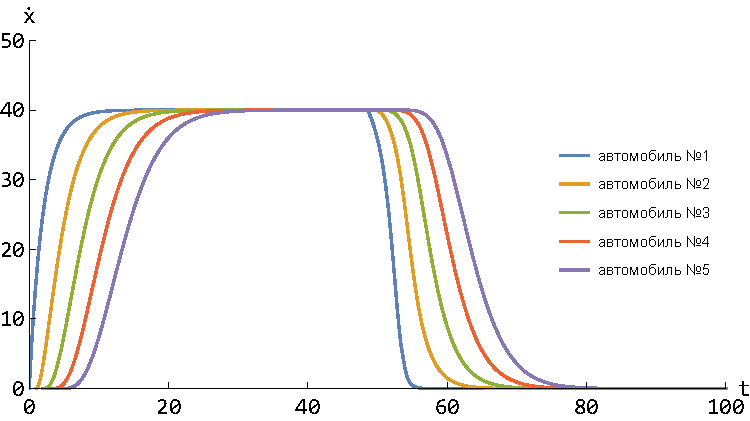
\includegraphics[width=1\linewidth,height=0.2\textheight]
			{Images/new_model_speed.pdf}
		\end{minipage}
		\hfill 
		\begin{minipage}[h!]{0.48\linewidth}
			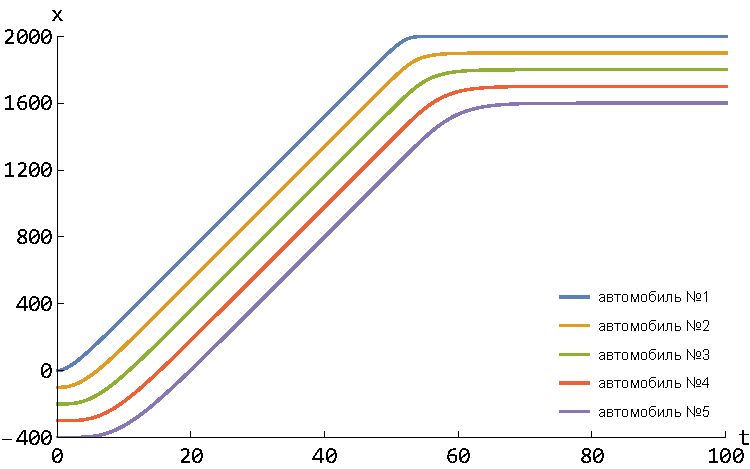
\includegraphics[width=1\linewidth,height=0.2\textheight]
			{Images/new_model_distanse.pdf}
		\end{minipage}
		\caption{Графики изменения скорости (слева) и расстояния (справа) для новой модели с параметрами: $a=0.5$, $q=0.6$, $v_{max}=40$, $v_{min}=0$, $\lambda=100$, $l=90$, $L=2000$, $x_0=0$, $v_n=0$, $g=9.8$, $\mu=0.6$. }
		\label{new_model_picture}
	\end{center}
\end{figure}

На графиках видна динамика, которая согласуется с динамикой реального транспортного потока. Автомобили разгоняются до максимальной допустимой скорости, двигаются с ней до момента начала торможения, затем начинают тормозить и останавливаются на безопасном расстоянии. 

Модель \eqref{my_model} согласуется с реальной наблюдаемой ситуацией только на небольшом расстоянии между транспортными средствами, так как на большом расстоянии автомобилю нет смысла подстраивать свою скорость под скорость впереди идущей машины. Введём понятие \textbf{``расстояние влияния''}, под которым будем понимать такое расстояние, начиная с которого впереди идущий автомобиль оказывает влияние на позади идущий. В качестве ``расстояние влияния'' можно взять двойной тормозной путь $2S$. Таким образом, если расстояние между автомобилями большем, чем  $2S$, то преследующий автомобиль старается максимизировать свою скорость, если меньше, чем  $2S$, то преследующий автомобиль подстраивает свою скорость относительно впереди идущего. Математически это можно записать в виде релейной функции:

\begin{equation*}
F(\Delta x_{n}(t,\tau))=
\begin{cases}
\begin{split}
&v_{max},\quad &\text{если }\Delta x_{n-1,n}(t,\tau) > 2\dfrac{\dot{x}_n^2(t)}{2\mu g}, \\
&\dot{x}_{n-1}(t-\tau),\quad &\text{если }\Delta x_{n-1,n}(t,\tau) \leq 2\dfrac{\dot{x}_n^2(t)}{2\mu g}.
\end{split}
\end{cases}
\end{equation*}

В реальной жизни максимальная комфортная скорость может быть своя у каждого автомобиля $v_{n,max}$, поэтому в некоторых случаях может возникнуть ситуация, когда впереди идущее транспортное средство движется со скоростью большей, чем максимальная комфортная скорость позади идущего. Для решения такой проблемы к первому слагаемому можно применить функцию Хевисайда \cite{Heaviside_function}, вида:
\begin{equation*}
\theta(\dot{x}_n(t))=
\begin{cases}
\begin{split}
&v_{n,max},\quad &\text{если }\dot{x}_n(t)>v_{n,max}, \\
&\dot{x}_n(t),\quad &\text{если }\dot{x}_n(t)>v_{n,max}.
\end{split}
\end{cases}
\end{equation*}

Полученная математическая модель транспортных потоков согласуется с динамикой реального транспортного потока, и описывает все автомобили, включая первый. Далее покажем её применение для описания реальной дорожной ситуации.

\section{Практическое применение новой математической модели} 

\subsection{Подбор параметров} 

Прежде чем применять новую математическую модель \eqref{new_model} для моделирования реального транспортного потока, введём систему единиц измерения для параметров, использующихся в модели.

Размерности для времени, расстояния и скорости возьмём из международной системы единиц (СИ). Таким образом, время будем измерять в секундах (с), расстояние в метрах (м), а скорость в метрах в секунду (м/с).

В системе \eqref{my_model} присутствуют параметры, значение которых можно определить заранее на основе физических законов, действующего законодательства Российской Федерации и логических соображений.

Параметр $v_{max}$ описывает максимальную желаемую скорость. В качестве максимального значения для параметра $v_{max}$ рассмотрим максимальную разрешённую скорость движения в населённом пункте \cite{PDD}, которая, согласно правилам дорожного движения, составляет 60 км/ч, что в системе СИ равняется примерно 16.7 м/с. Таким образом, $v_{max} \in [0,16.7]$. Параметр $v_{min}$ описывает минимальную желаемую скорость и ограничен лишь параметром $v_{max}$, таким образом, $v_{min} \in [0,v_{max}]$. В дорожных ситуациях данные параметры будут иметь конкретные значения.

Параметр $\lambda$, который описывает начальное расстояние между двумя соседними автомобилями, будем считать равным 3 метра \cite{PDD}, а параметр $l$ возьмём равным 2 метра.

Параметр $\tau$, который описывает время реакции водителя, будем считать равным 1 секунде \cite{PDD}.

Коэффициент трения $\mu$ возьмём равный коэффициенту трения шин автомобиля по сухому асфальту $0.6$ \cite{Physics}.

Ускорение свободного падения $g$ на поверхности Земли равно приблизительно $9.8 \text{ м/с}^2$.

Параметры $a$ и $q$ являются вычисляемыми и не имеют размерности. Подберём эти параметры эмпирически, исходя из наблюдаемых закономерностей. В городских условиях автомобиль разгоняется до скорости 60 км/ч в среднем за 7 с, такое ускорение достигается при $a\approx1$. Автомобиль, сбрасывая скорость до полной остановки, должен проехать расстояние равное тормозному пути, это достигается при $q\approx1$. Таким образом, возьмём коэффициенты $a$ и $q$ равными $1$.

Начальные параметры, такие как расстояние до препятствия $L$, начальное положение первого автомобиля $\lambda_0$, начальные скорости автомобилей потока $v_n$ могут быть любыми, так как они зависят от конкретной дорожной ситуации и не влияют на динамику движения транспортного потока.

Объединим все полученные параметры и запишем их в виде таблицы \ref{real_parameters}.
\begin{table}[h!]
	\caption{Значения константных параметров для модели \eqref{new_model} }
	\label{real_parameters}
	\begin{center}
		\begin{tabularx}{\textwidth}{p{0.12\linewidth}p{0.52\linewidth}p{0.11\linewidth}p{0.15\linewidth}}			
			\hline
			\rule{0cm}{0,5cm}
			Символ & Описание & Значение & Единица СИ \\
			[3pt]\hline
			$v_{max}$ & максимальная желаемая скорость& $[0,16.7]$&м/с\\
			$v_{min}$ & минимальная желаемая скорость& $[0,v_{max}]$&м/с\\ 
			$\tau$ & время реакции водителя& 1&с\\
			$\lambda$ & начальное расстояние между автомобилями& 3&м\\
			$l$ & расстояние между автомобилями& 2&м\\
			$g$ & ускорение свободного падения& 9.8&$\text{м/с}^2$\\ 
			$\mu$ & коэффициент трения& 0.6& безразмерная\\ 
			$a$ & коэффициент ускорения& 1& безразмерная\\
			$q$ & коэффициент торможения& 1& безразмерная\\
			\hline
		\end{tabularx}
	\end{center}
\end{table}
\newline 

\subsection{Применение новой математической модели в некоторых дорожных ситуациях}

Для моделирования некоторых реальных дорожных ситуаций были использованы компьютерные технологии, а именно была написана программа на языке программирования $Python$ версии 3.8.2 \cite{Python}. Также были проведены наблюдения за реальными светофорами. Результаты наблюдений представлены в приложении \ref{att}.

Автомобили в приложении двигаются согласно математической модели \eqref{my_model} с параметрами из таблицы \ref{real_parameters}. Для решения системы дифференциальных уравнений с запаздыванием в программе используется метод Рунге-Кутты \cite{Runge_Kutta}, адаптированный для уравнений с запаздыванием.

В начальный момент времени все автомобили стоят на безопасном расстоянии друг от друга. Началом отсчёта пройденного пути считается начальное положение первого автомобиля, таким образом, автомобили, которые не доехали до начального положения первого автомобиля, имеют отрицательное значение пройденного пути.

В модели \eqref{my_model} транспортные средства считались материальными точками и их размеры не учитывались, но для большей реалистичности в программе были использованы схематичные изображения автомобилей, которые, как и реальные транспортные средства, имеют размер. В данном случае габариты автомобиля равняются размеру его изображения. Эта величина прибавлена к константам $\lambda$ и $l$ и не оказывает влияния на динамику движения.

Полученная программа имеет три режима работы, каждый из которых позволяет смоделировать поведение автомобилей в конкретной дорожной ситуации. Для каждого режима есть свой набор начальных данных. ``Количество машин'' и ``максимальная скорость'' являются общими параметрами и указываются для каждого режима.

\noindent Таким образом, с помощью программы можно смоделировать:

\begin{itemize} 
	\item \textit{начало движения и остановку автомобилей},
	\item \textit{режим работы одного светофора},
	\item \textit{режим работы двух светофоров}.
\end{itemize}

\noindent Рассмотрим каждый режим работы программы в отдельности.

\subsubsection{Начало движения и остановка}

Первый режим работы программы --- это моделирование двух простых дорожных ситуаций, а именно, начало движения автомобиля и его торможение или остановка. Эти дорожные ситуации использовались для демонстрации применения всех моделей, рассмотренных в данной работе.

В этом режиме работы программы задаётся дистанция, по достижению которой, автомобили должны сбросить скорость и значение минимальной скорости, до которой автомобили сбросят свою текущую скорость. В случае указания нулевого значения минимальной скорости машины остановятся.

На рисунках \ref{first_mode_1} --- \ref{first_mode_4} изображены этапы работы программы в первом режиме.

\begin{figure}[h!]
	\begin{center}
		\begin{minipage}[h]{0.48\linewidth}
			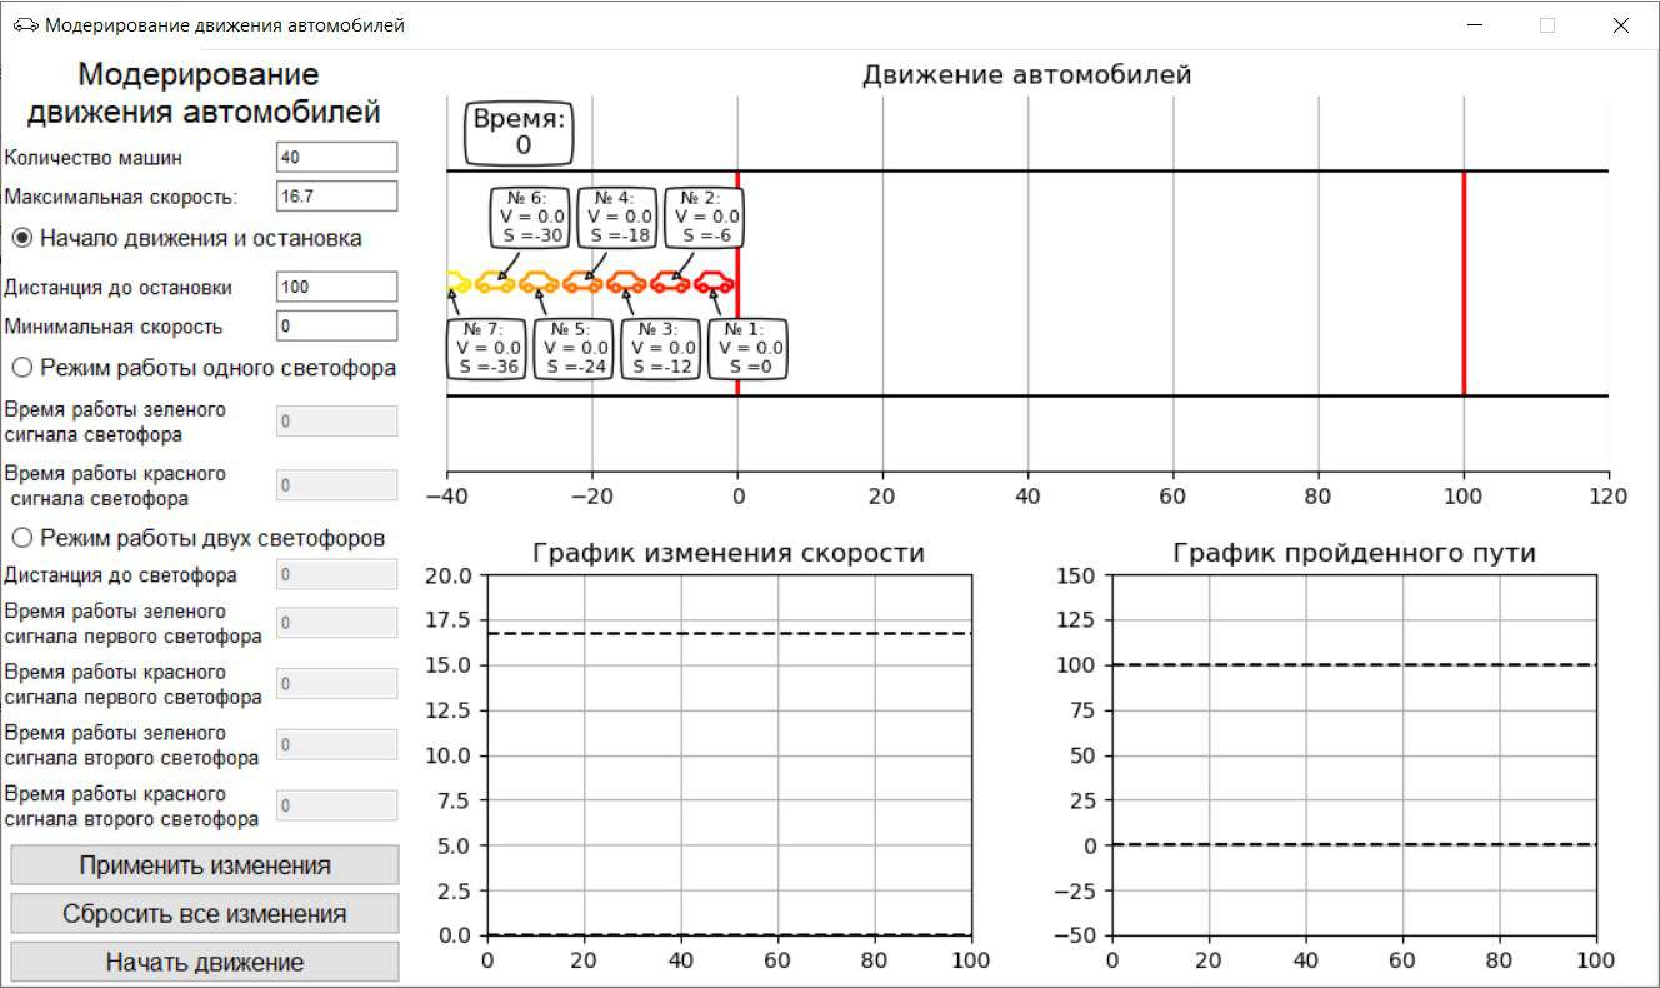
\includegraphics[width=1\linewidth]
			{Images/screens/first_mode_1}
			\caption{Положение автомобилей в нулевой момент времени.} 
			\label{first_mode_1}
		\end{minipage}
		\hfill 
		\begin{minipage}[h]{0.48\linewidth}
			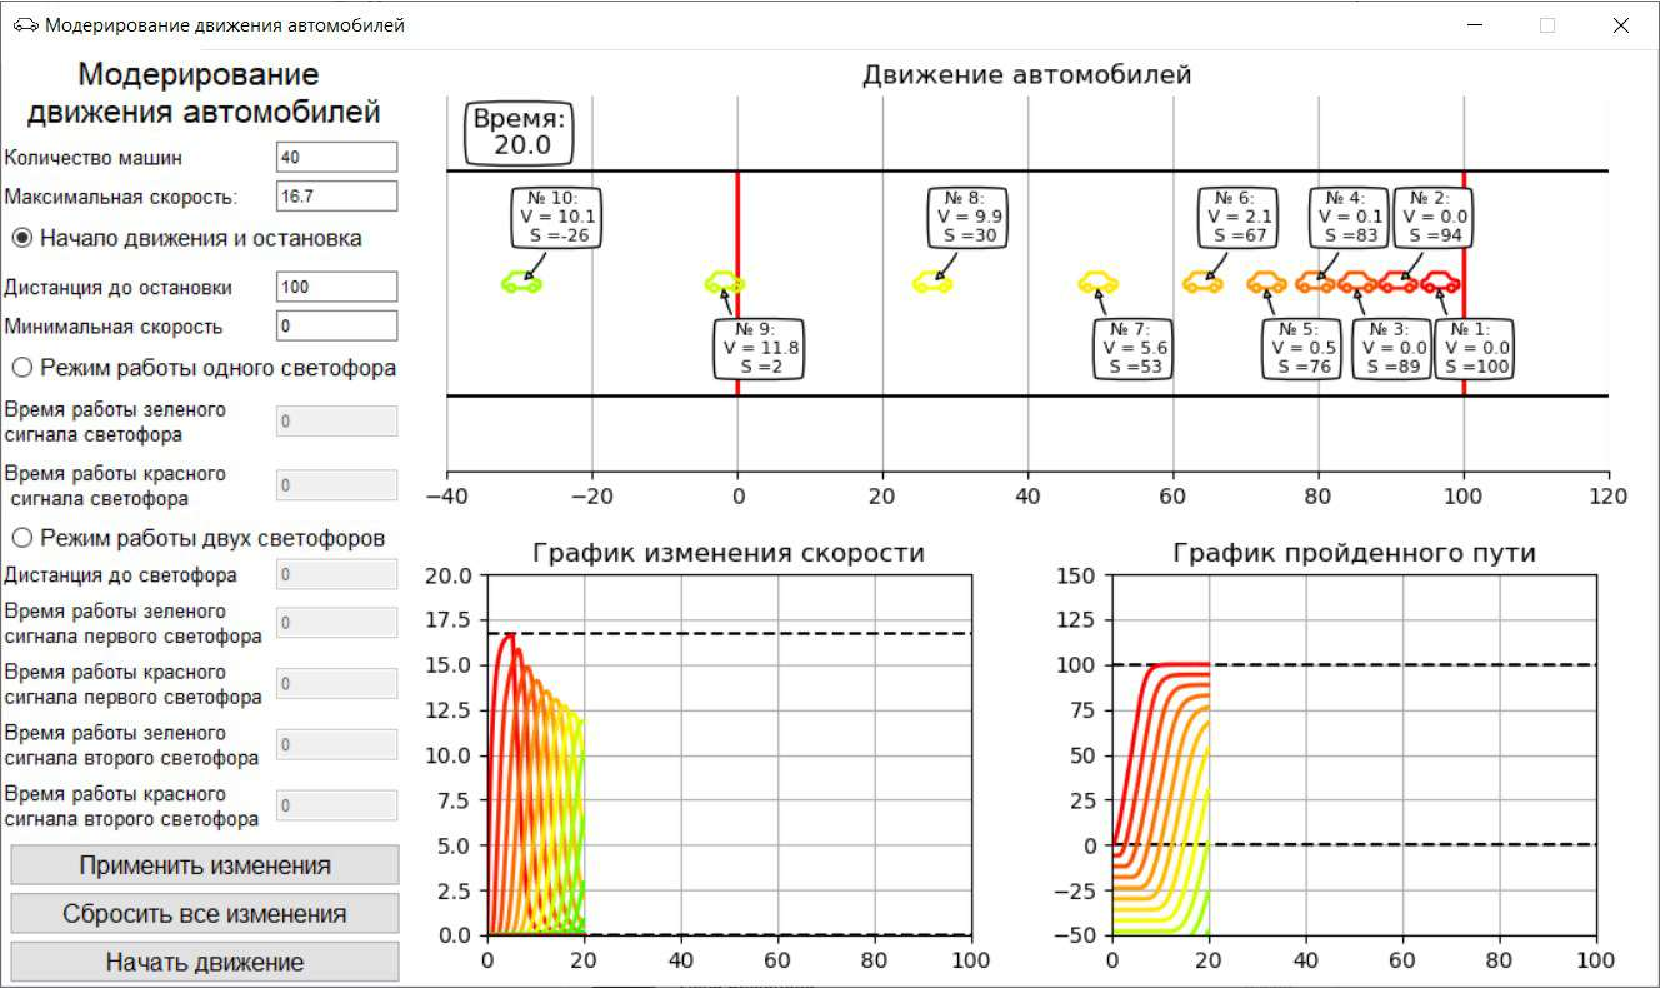
\includegraphics[width=1\linewidth]
			{Images/screens/first_mode_2}
			\caption{Положение автомобилей через 20 секунд после начала движения.}
			\label{first_mode_2}
		\end{minipage}
		\hfill 
		\begin{minipage}[h]{0.48\linewidth}
			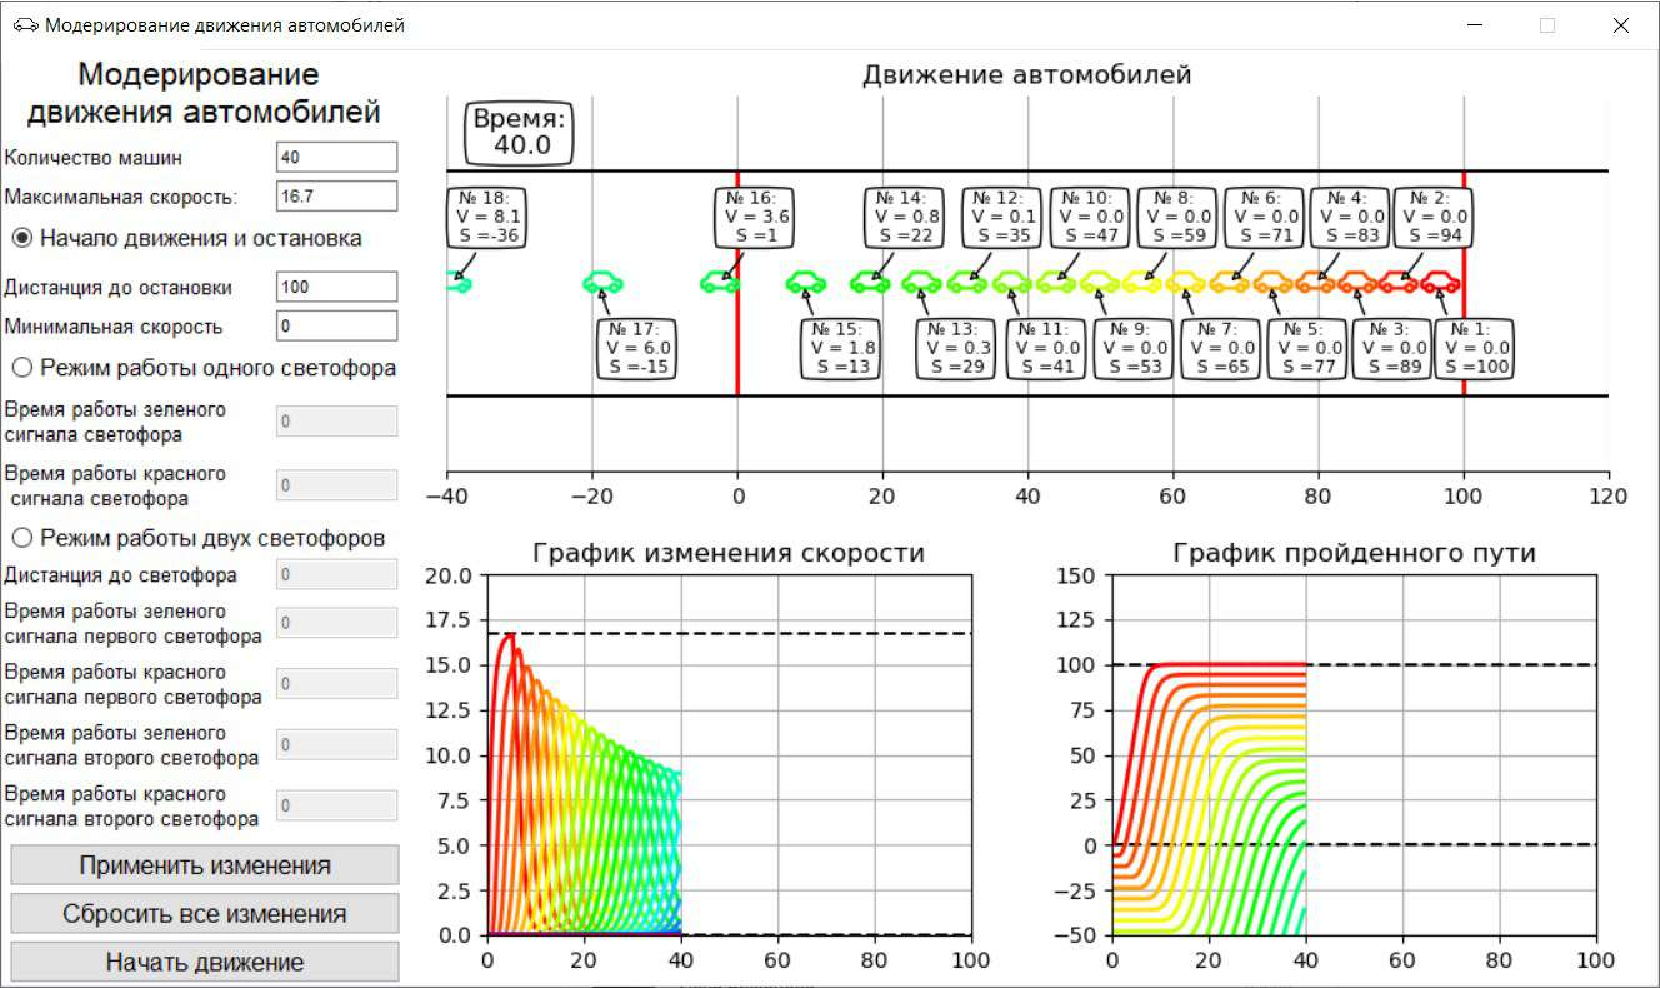
\includegraphics[width=1\linewidth]
			{Images/screens/first_mode_3}
			\caption{Положение автомобилей через 40 секунд после начала движения.}
			\label{first_mode_3}
		\end{minipage}
			\hfill 
		\begin{minipage}[h]{0.48\linewidth}
			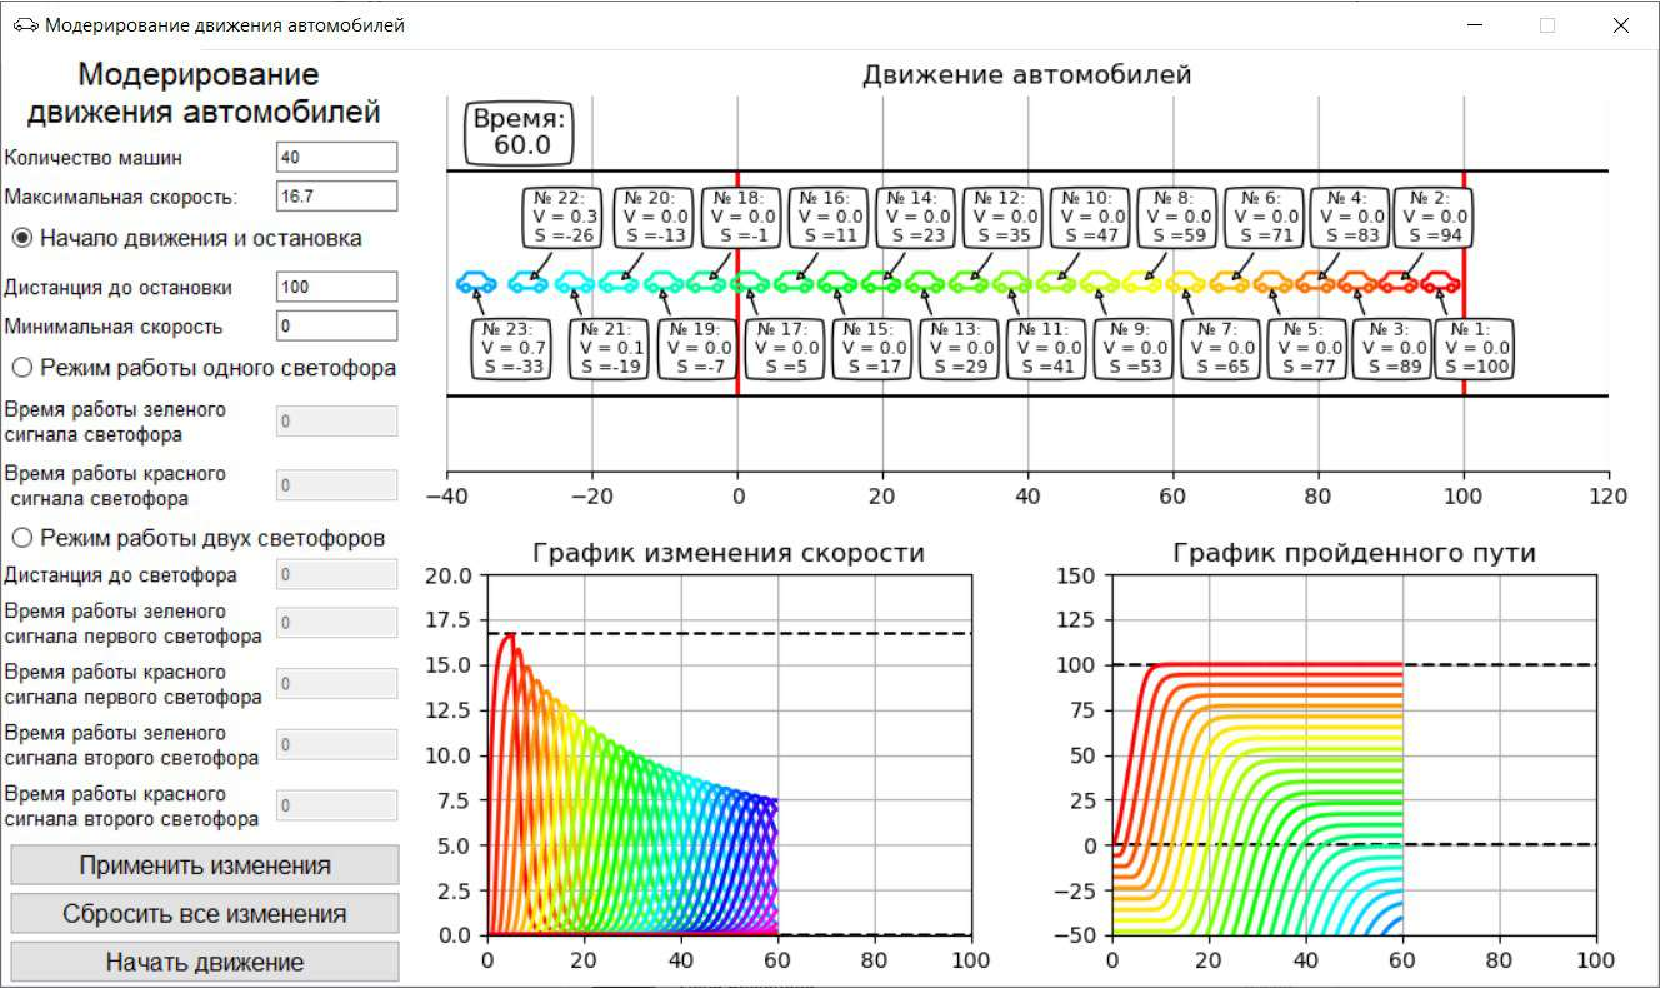
\includegraphics[width=1\linewidth]
			{Images/screens/first_mode_4}
			\caption{Положение автомобилей через 60 секунд после начала движения.}
			\label{first_mode_4}
		\end{minipage}
	\end{center}
\end{figure}

Из рисунков видно, что работа программы в данном режиме полностью согласуется с динамикой реального транспортного потока.

Данный режим работы программы подойдёт для моделирования участков дорог, где присутствует изменение скоростного режима.

\subsubsection{Режим работы одного светофора}

Второй режим работы программы --- это моделирование режима работы одного светофора. Работа светофора состоит из циклов, которые в свою очередь состоят из двух фаз. Первая фаза определяется временным интервалом работы зелёного сигнала светофора, а вторая --- красного. В данном режиме работы программы задаются временные интервалы работы зелёного и красного сигналов светофора. 

Во время работы зелёного сигнала светофора автомобили проезжают через светофор, во время работы красного сигнала автомобили останавливаются перед светофором на безопасном расстоянии и ждут включения зелёного сигнала. 

Основным критерием работы светофора будем считать количество автомобилей, которые проехали через светофор за один цикл его работы, а именно за время работы зелёного сигнала. Иногда может возникнуть ситуация, когда в момент смены сигнала светофора расстояние между автомобилем и светофором меньше, чем длинна тормозного пути. В таком случае, чтобы не применять экстренное торможение, автомобилю разрешается проехать светофор на запрещающий сигнал. Такое поведение согласуется с правилами дорожного движения \cite{PDD}.

На рисунках \ref{second_mode_1} --- \ref{second_mode_9} показано применение программы для моделирования работы одного светофора, с характеристиками, наблюдаемыми у реального светофора.

\begin{figure}[h!]
	\begin{center}
		\begin{minipage}[h]{0.48\linewidth}
			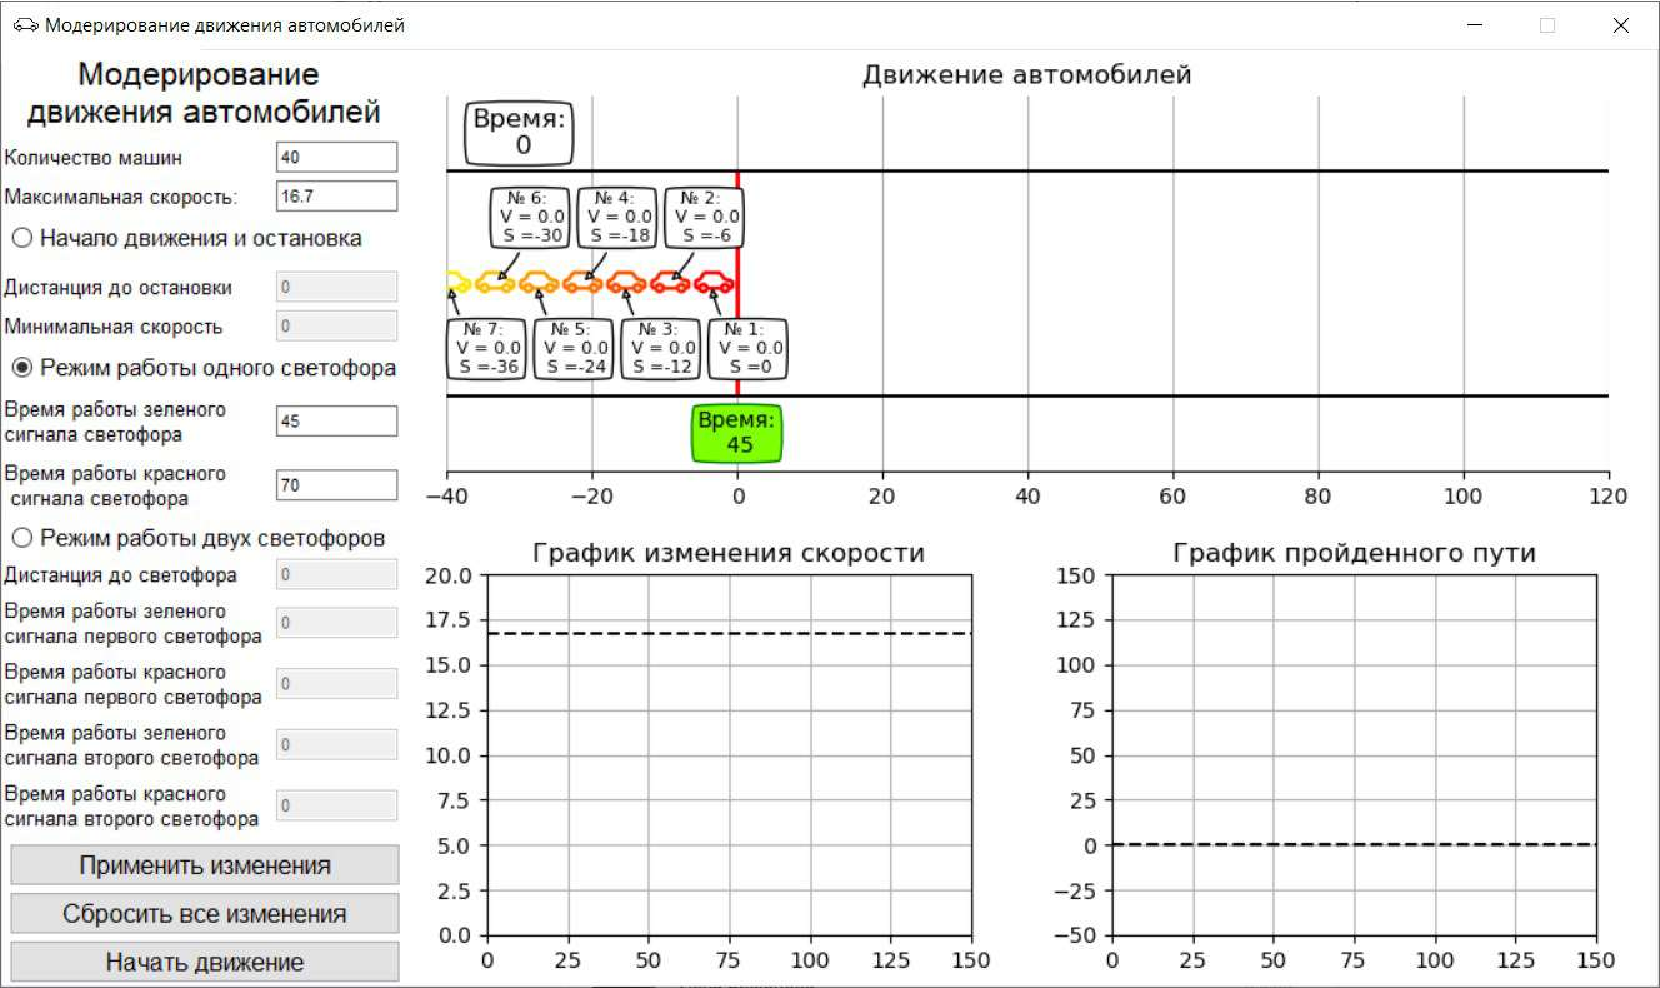
\includegraphics[width=1\linewidth]
			{Images/screens/second_mode_1}
			\caption{Положение автомобилей в нулевой момент времени.} 
			\label{second_mode_1}
		\end{minipage}
		\hfill 
		\begin{minipage}[h]{0.48\linewidth}
			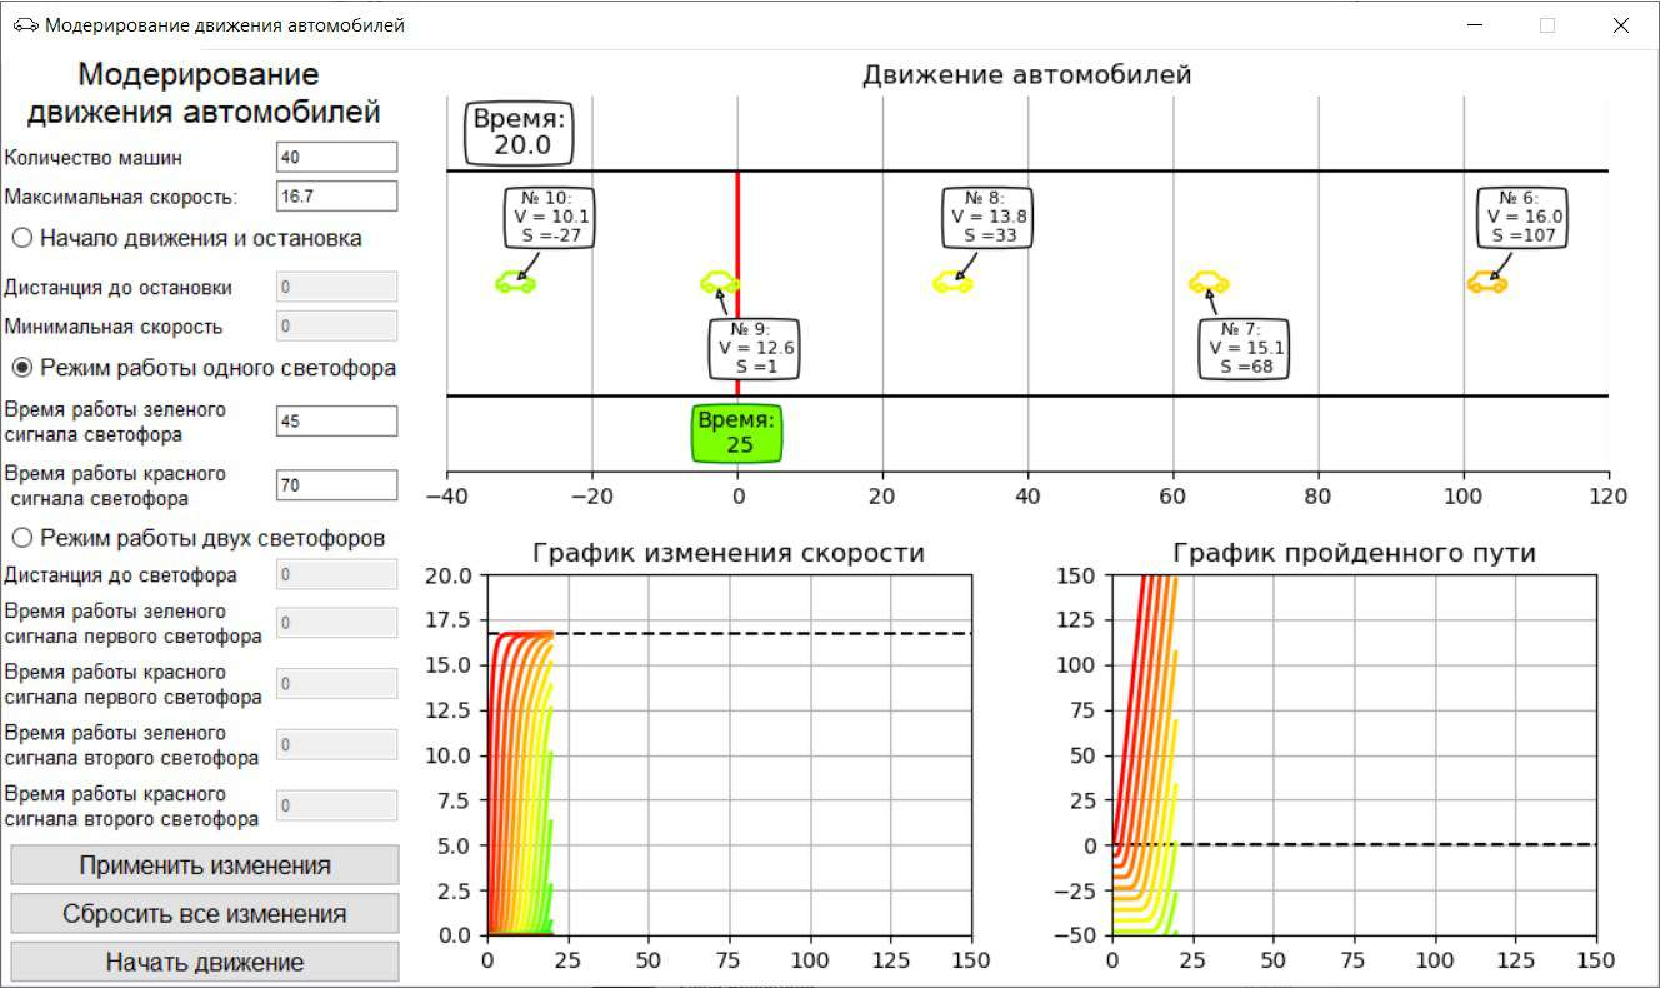
\includegraphics[width=1\linewidth]
			{Images/screens/second_mode_2}
			\caption{Положение автомобилей через 20 секунд после начала движения.}
			\label{second_mode_2}
		\end{minipage}
	\end{center}
\end{figure}
\begin{figure}[h!]
	\begin{center}
		\begin{minipage}[h]{0.48\linewidth}
			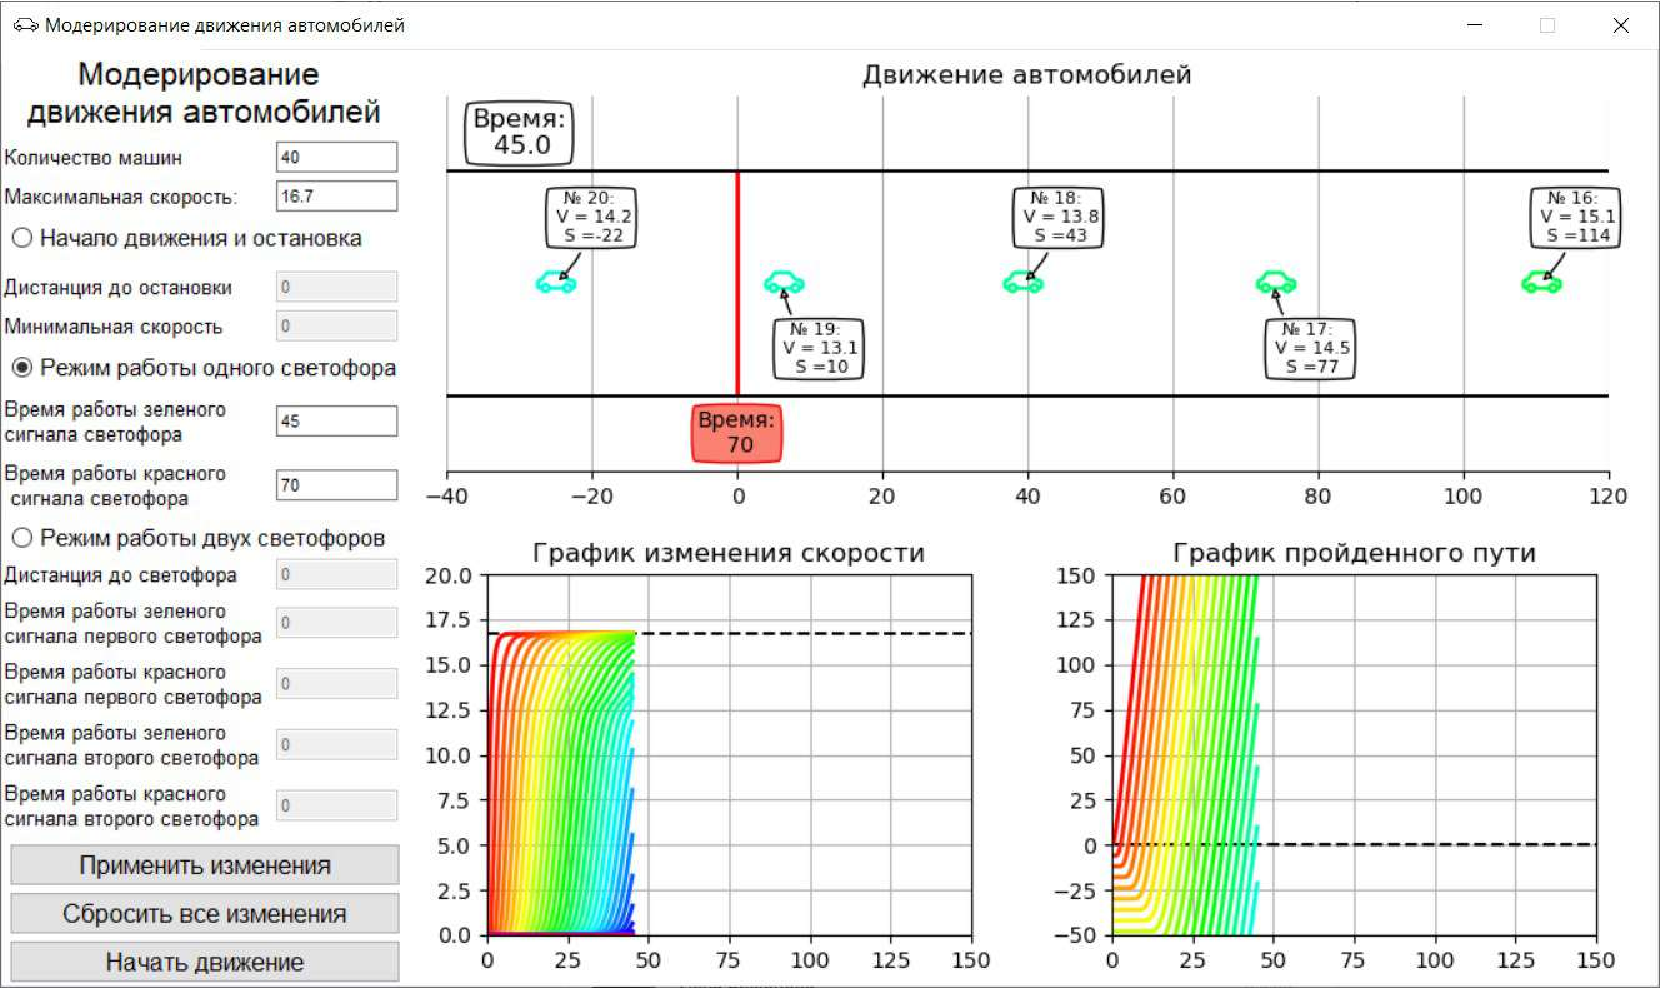
\includegraphics[width=1\linewidth]
			{Images/screens/second_mode_3}
			\caption{Положение автомобилей через 45 секунд после начала движения.}
			\label{second_mode_3}
		\end{minipage}
		\hfill 
		\begin{minipage}[h]{0.48\linewidth}
			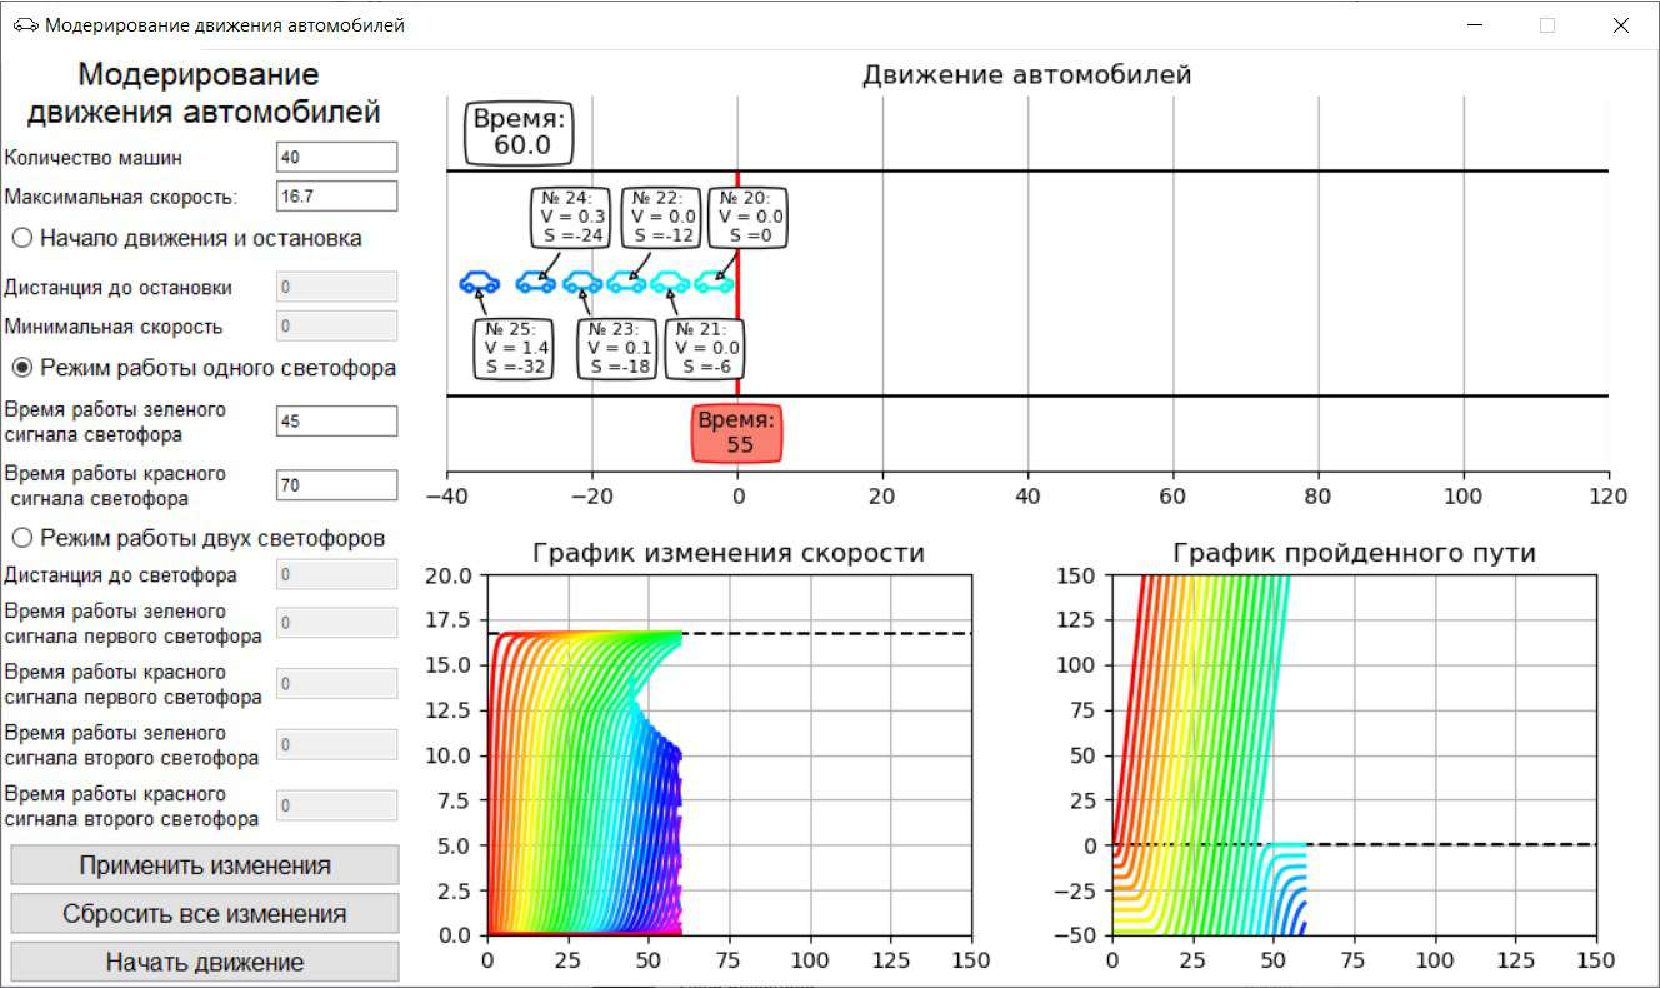
\includegraphics[width=1\linewidth]
			{Images/screens/second_mode_4}
			\caption{Положение автомобилей через 60 секунд после начала движения.}
			\label{second_mode_4}
		\end{minipage}
		\hfill
		\begin{minipage}[h]{0.48\linewidth}
			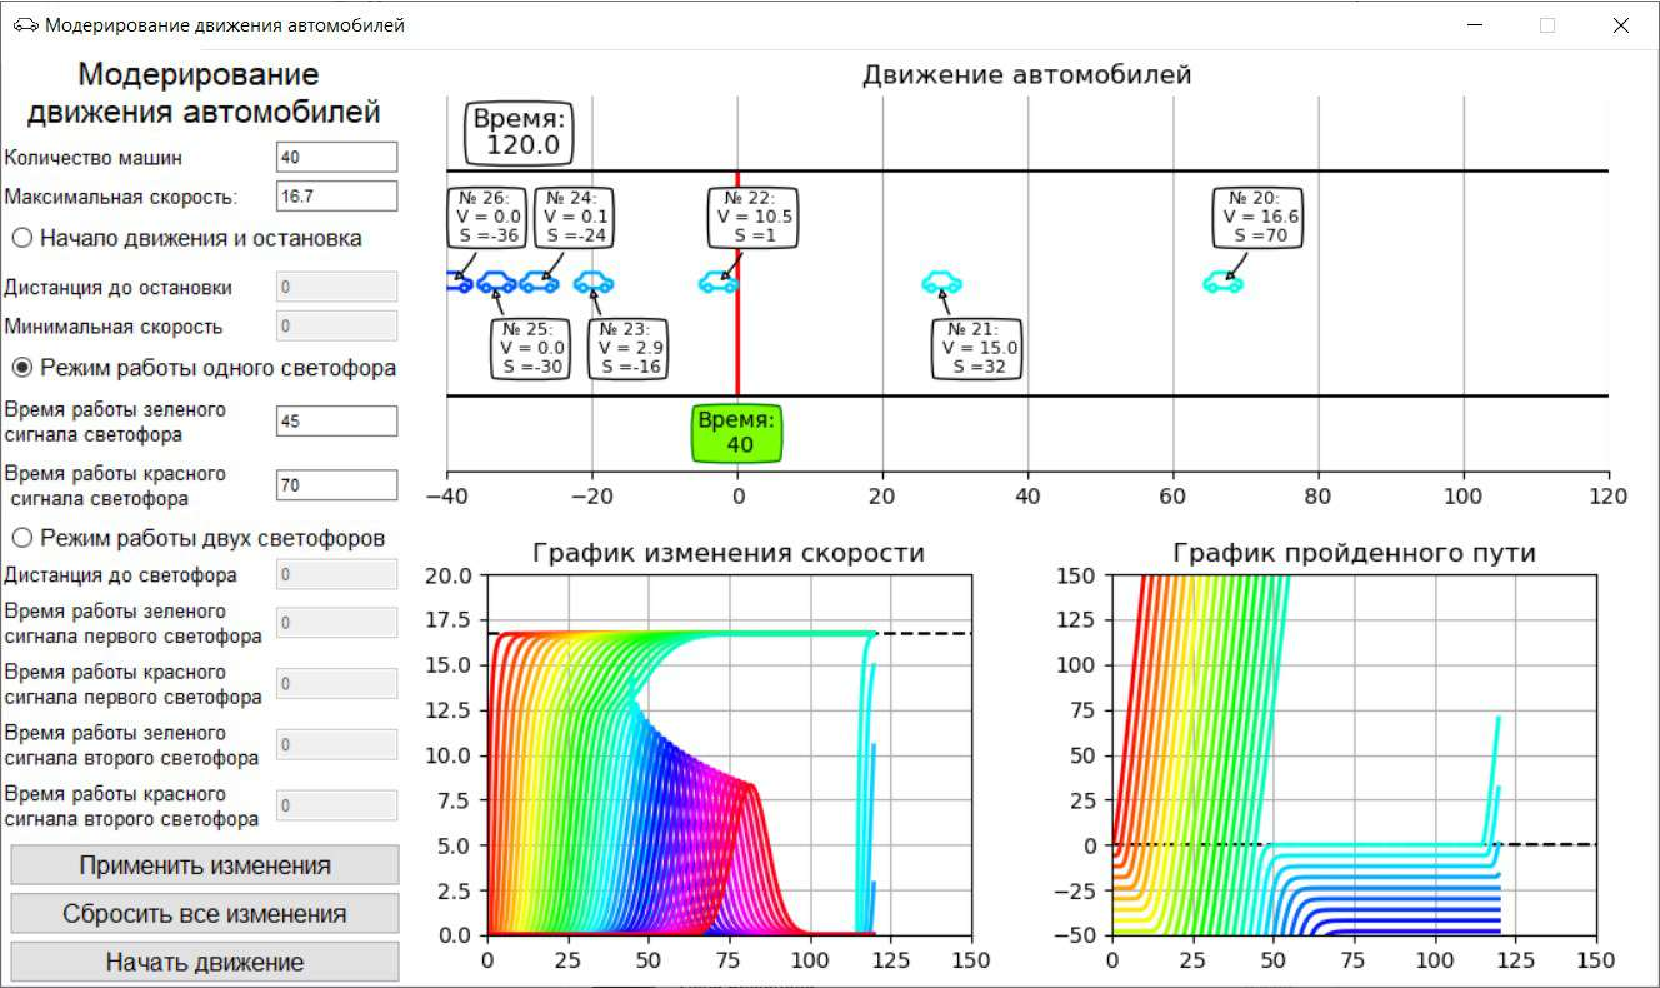
\includegraphics[width=1\linewidth]
			{Images/screens/second_mode_6}
			\caption{Положение автомобилей через 120 секунд после начала движения.}
			\label{second_mode_6}
		\end{minipage}
		\hfill
		\begin{minipage}[h]{0.48\linewidth}
			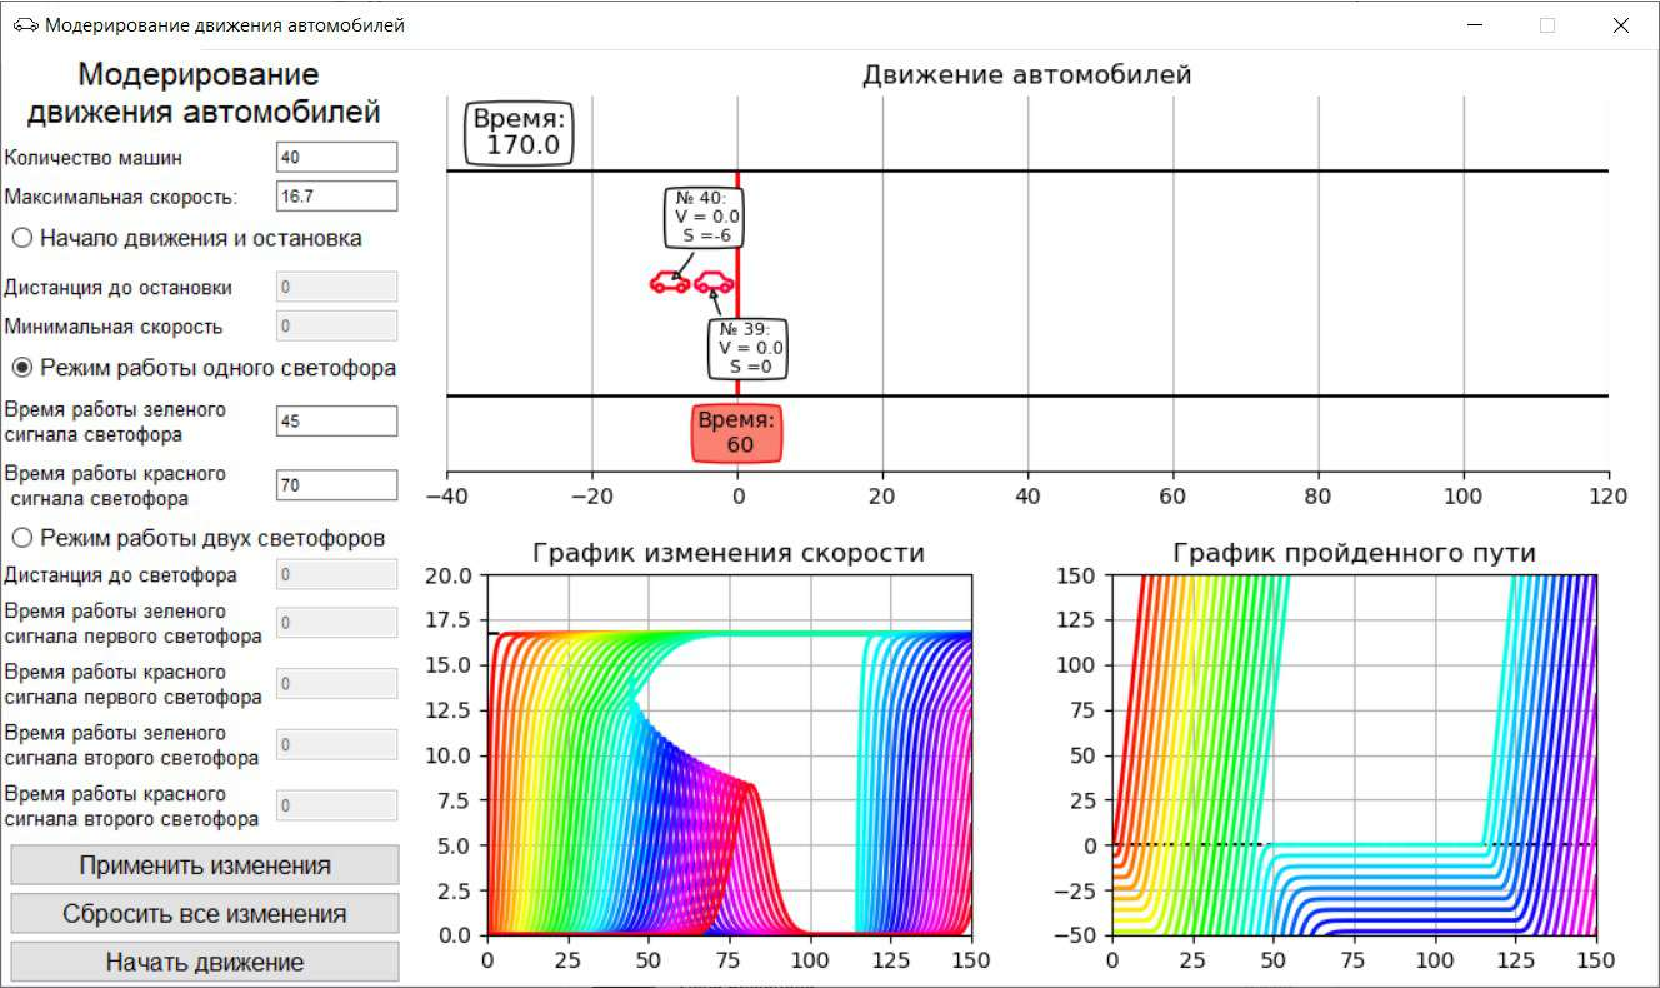
\includegraphics[width=1\linewidth]
			{Images/screens/second_mode_9}
			\caption{Положение автомобилей через 170 секунд после начала движения.} 
			\label{second_mode_9}
		\end{minipage}
	\end{center}
\end{figure}

На рисунках \ref{second_mode_1} --- \ref{second_mode_9} показано моделирование нескольких циклов работы реального светофора. Как видно из рисунков количество автомобилей, которые проезжают через светофор в разработанном приложении равно среднему количеству автомобилей, которые проезжают через реальный светофор (приложение \ref{att}). Это подтверждает корректность и самой модели \eqref{my_model}, и правильность подбора параметров (таблица \ref{real_parameters}). 

Данный режим работы программы подойдёт для моделирования участков дорог со светофором. С его помощью можно отрегулировать режим работы светофора не опасаясь серьёзных последствий, таких как пробки, которые могли бы возникнуть при неудачной настройке реального светофора.  

\subsubsection{Режим работы двух светофоров}

Третий режим программы --- это моделирование режима работы двух последовательно идущих светофоров. Светофоры в данном режиме не зависят друг от друга и работа каждого из них аналогична работе светофора, рассмотренной в предыдущем пункте. Соответственно, поведение автомобилей также остаётся аналогичным случаю одного светофора.

В данном режиме задаётся время работы зелёного и красного сигналов для каждого светофора и расстояние между ними. 

На рисунках \ref{third_mode_1} --- \ref{third_mode_15} показано применение программы для моделирования работы двух последовательно идущих светофоров, с характеристиками, наблюдаемыми у двух реальных светофоров, идущих друг за другом (приложение \ref{att}).

\begin{figure}[H]
	\begin{center}
		\begin{minipage}[h]{0.48\linewidth}
			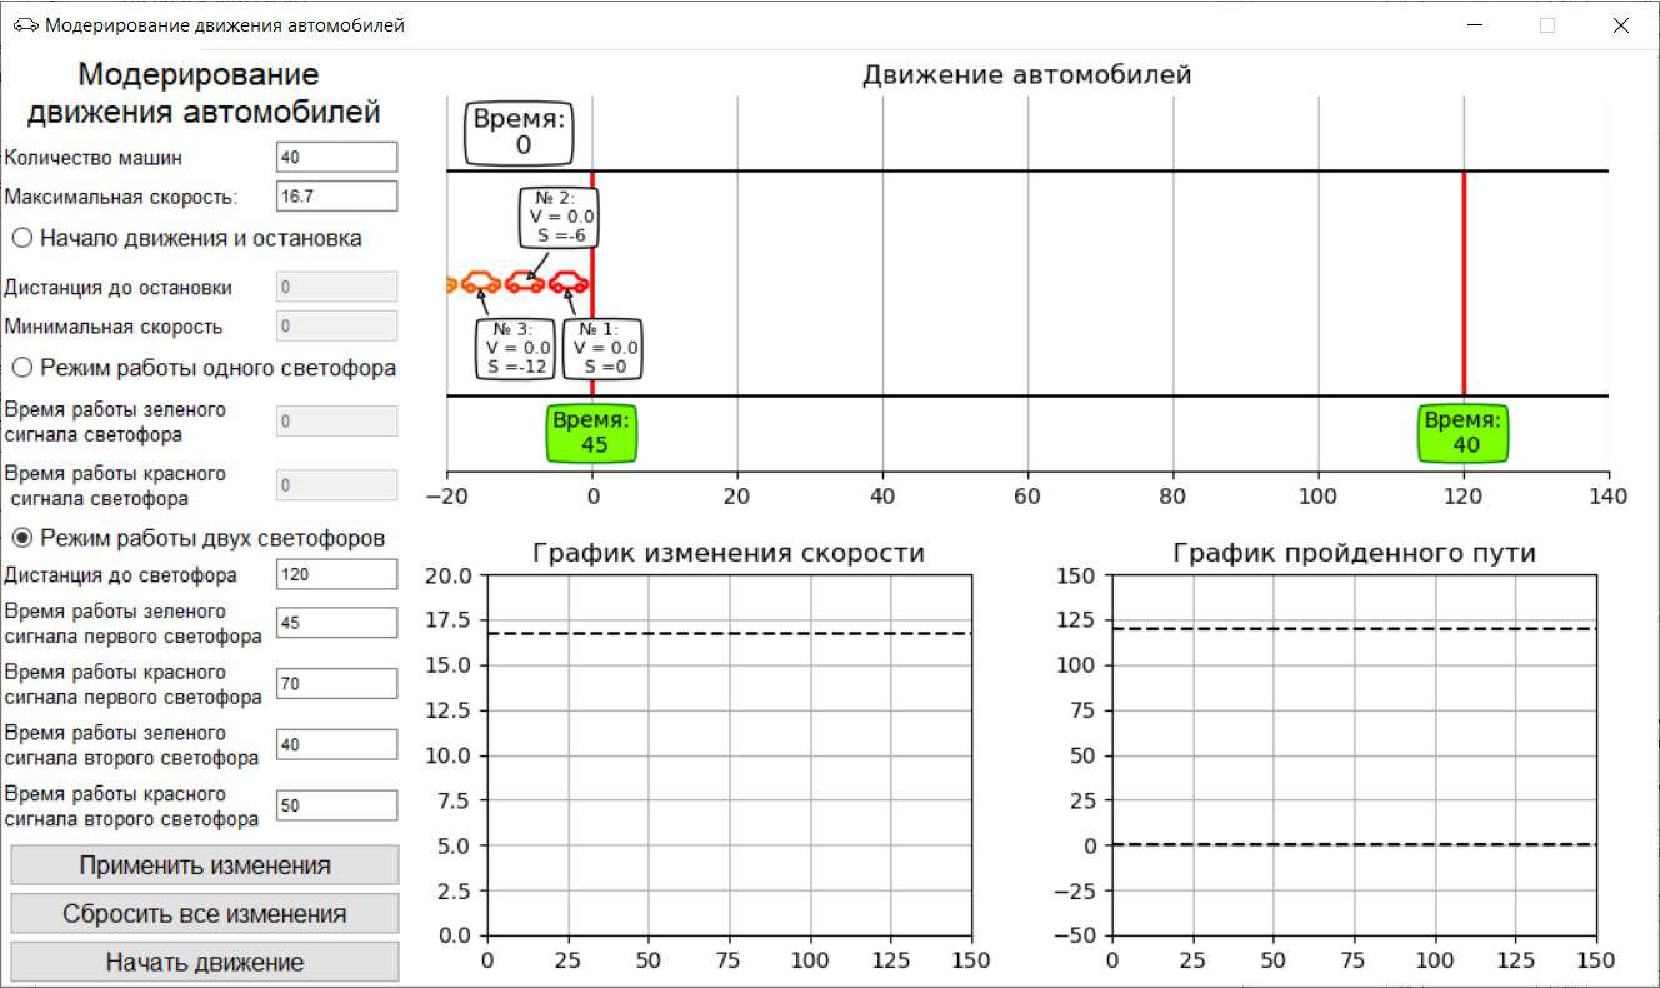
\includegraphics[width=1\linewidth]
			{Images/screens/third_mode_1}
			\caption{Положение автомобилей в нулевой момент времени.} 
			\label{third_mode_1}
		\end{minipage}
		\hfill 
		\begin{minipage}[h]{0.48\linewidth}
			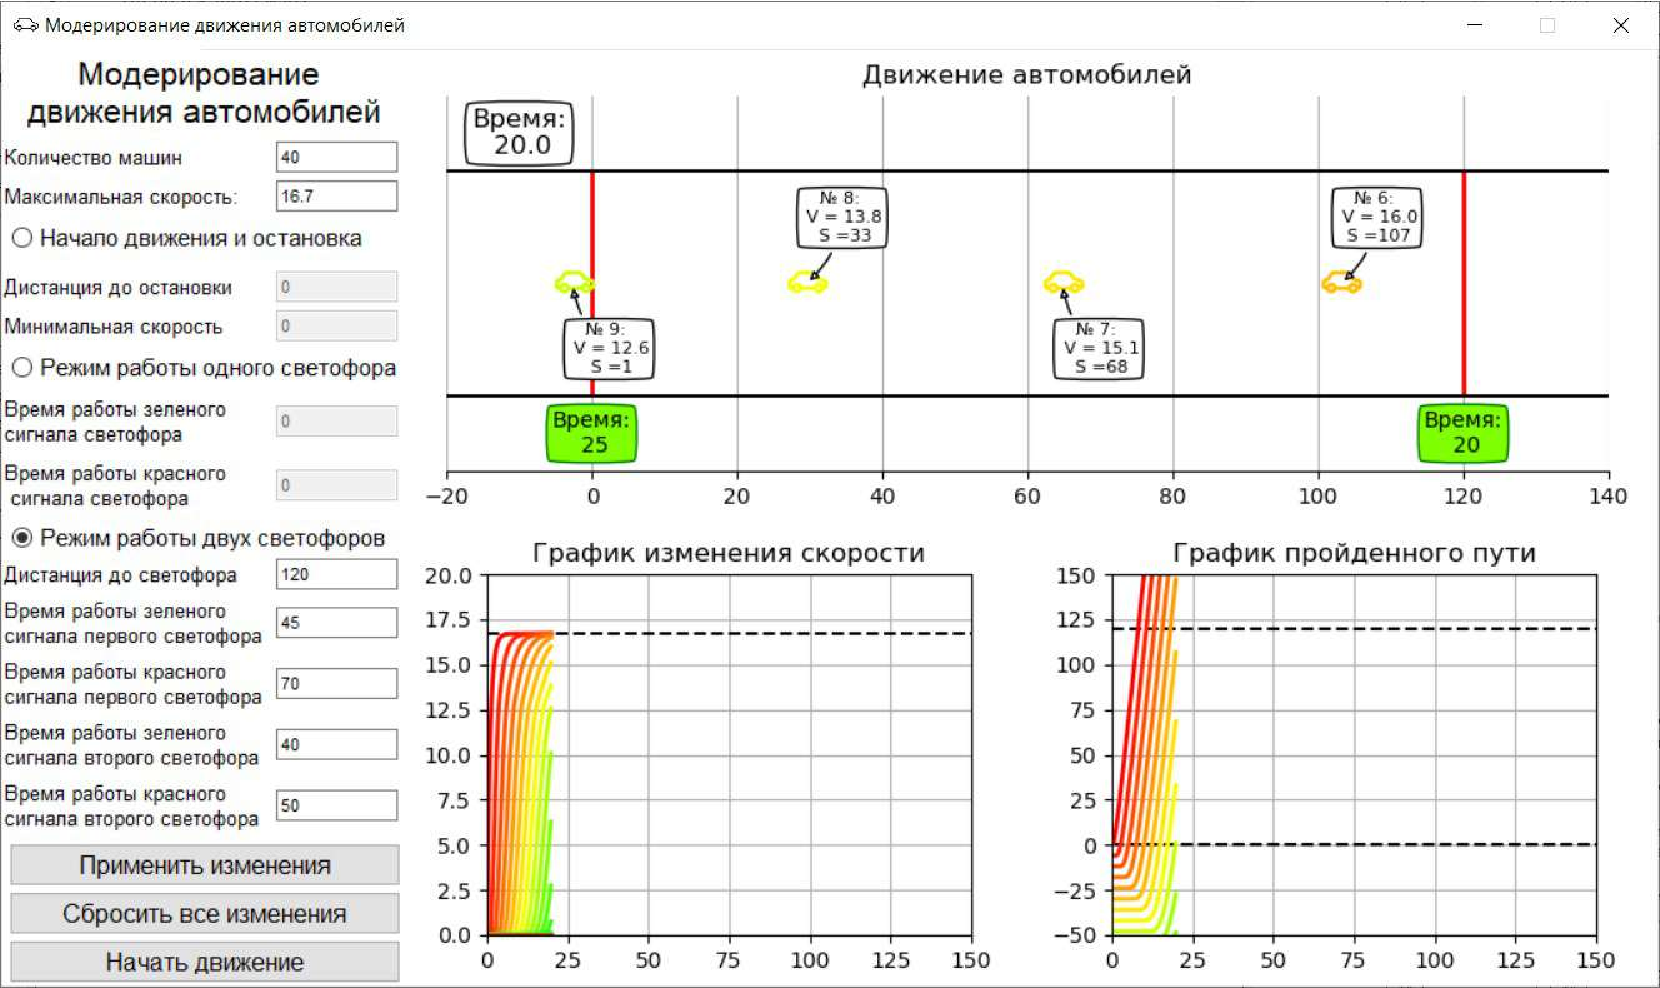
\includegraphics[width=1\linewidth]
			{Images/screens/third_mode_2}
			\caption{Положение автомобилей через 20 секунд после начала движения.}
			\label{third_mode_2}
		\end{minipage}
	\end{center}
\end{figure}

\begin{figure}[H]
	\begin{center}	 
		\begin{minipage}[h]{0.48\linewidth}
			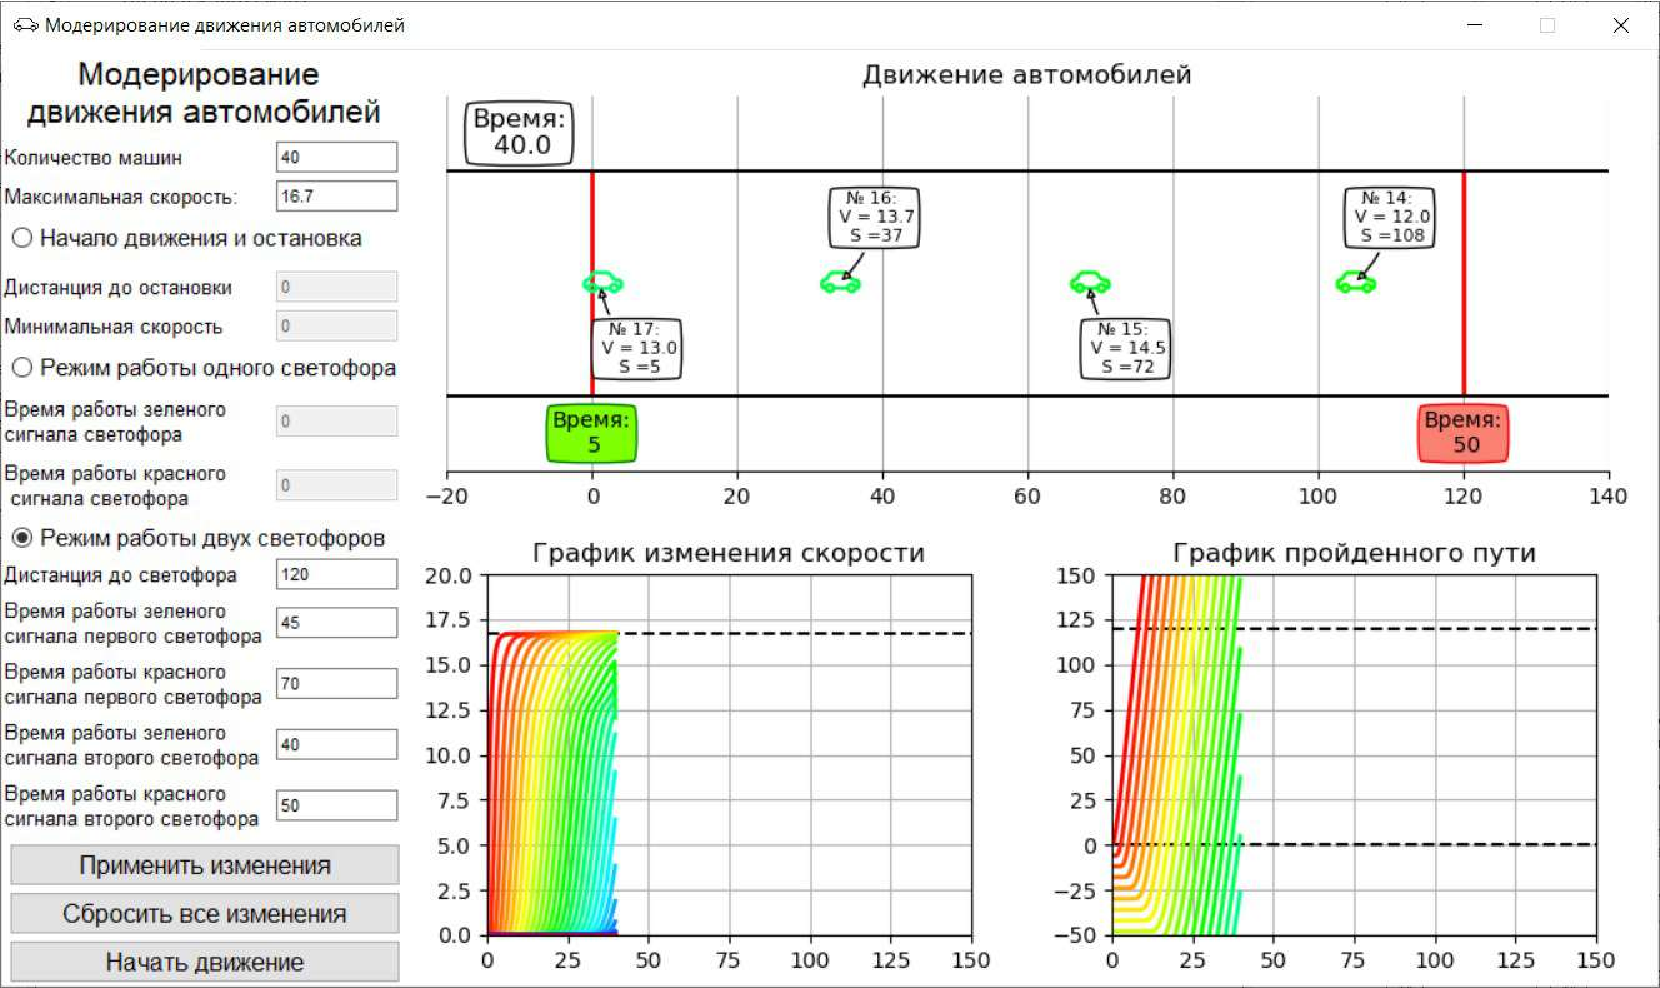
\includegraphics[width=1\linewidth]
			{Images/screens/third_mode_3}
			\caption{Положение автомобилей через 40 секунд после начала движения.}
			\label{third_mode_3}
		\end{minipage}
		\hfill 
		\begin{minipage}[h]{0.48\linewidth}
			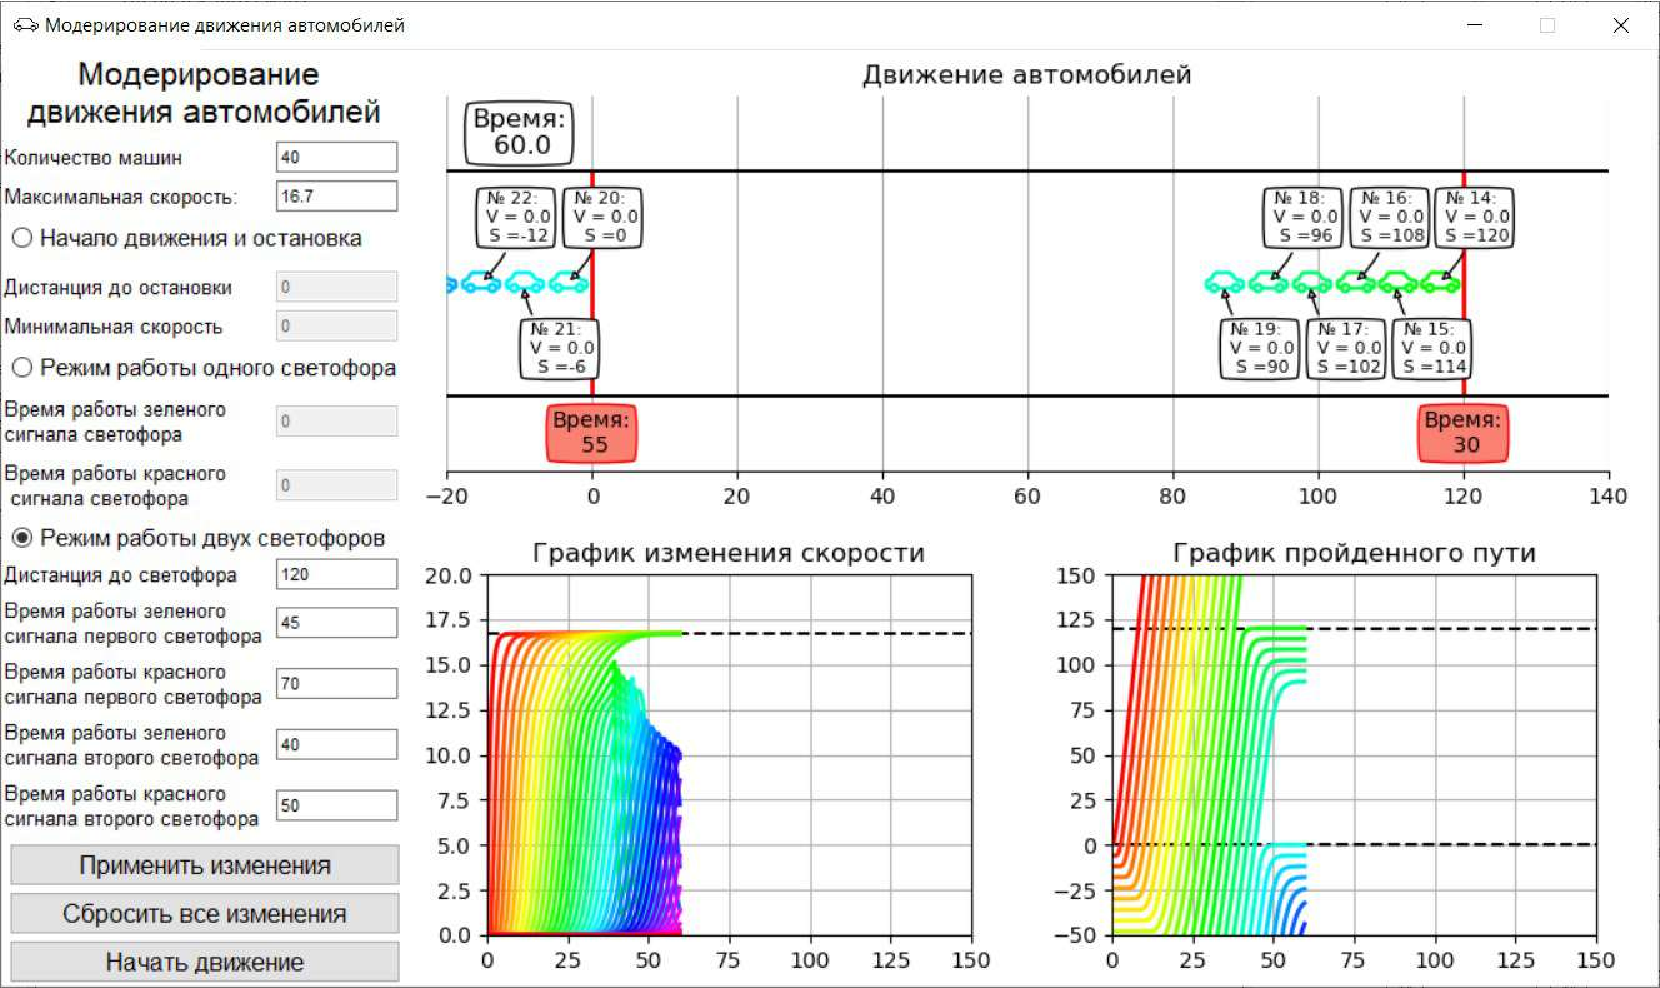
\includegraphics[width=1\linewidth]
			{Images/screens/third_mode_4}
			\caption{Положение автомобилей через 60 секунд после начала движения.}
			\label{third_mode_4}
		\end{minipage}
		\hfill
		\begin{minipage}[h]{0.48\linewidth}
			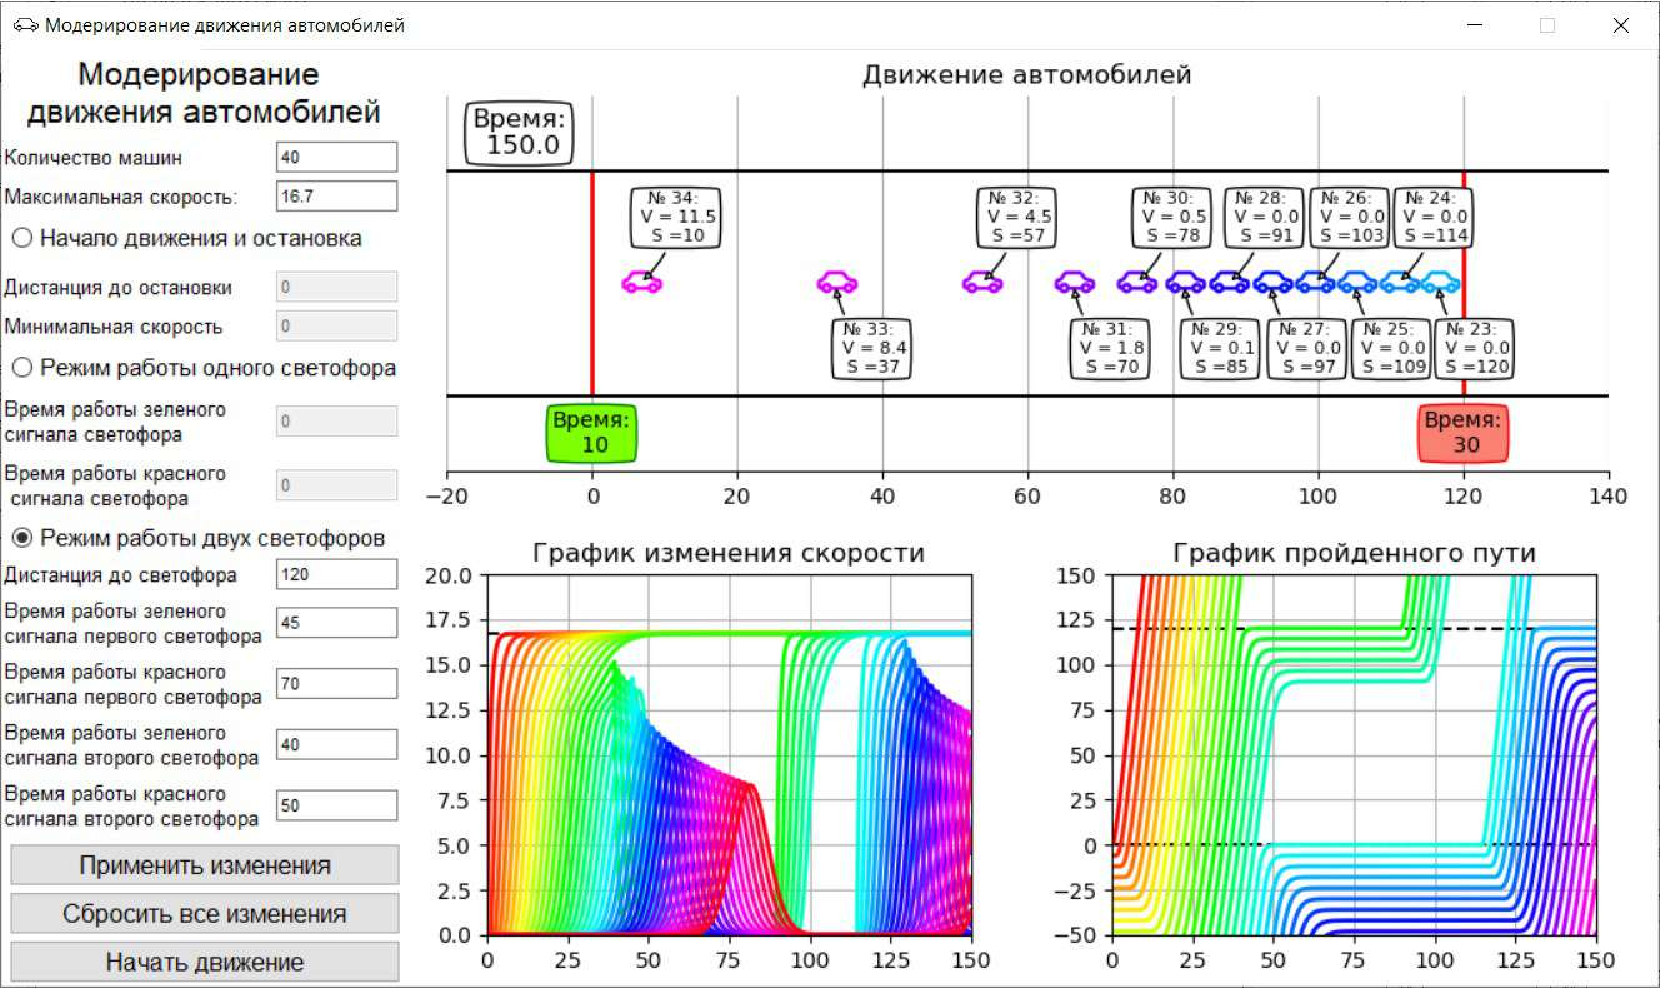
\includegraphics[width=1\linewidth]
			{Images/screens/third_mode_11}
			\caption{Положение автомобилей через 150 секунд после начала движения.}
			\label{third_mode_11}
		\end{minipage}
		\hfill 
		\begin{minipage}[h]{0.48\linewidth}
			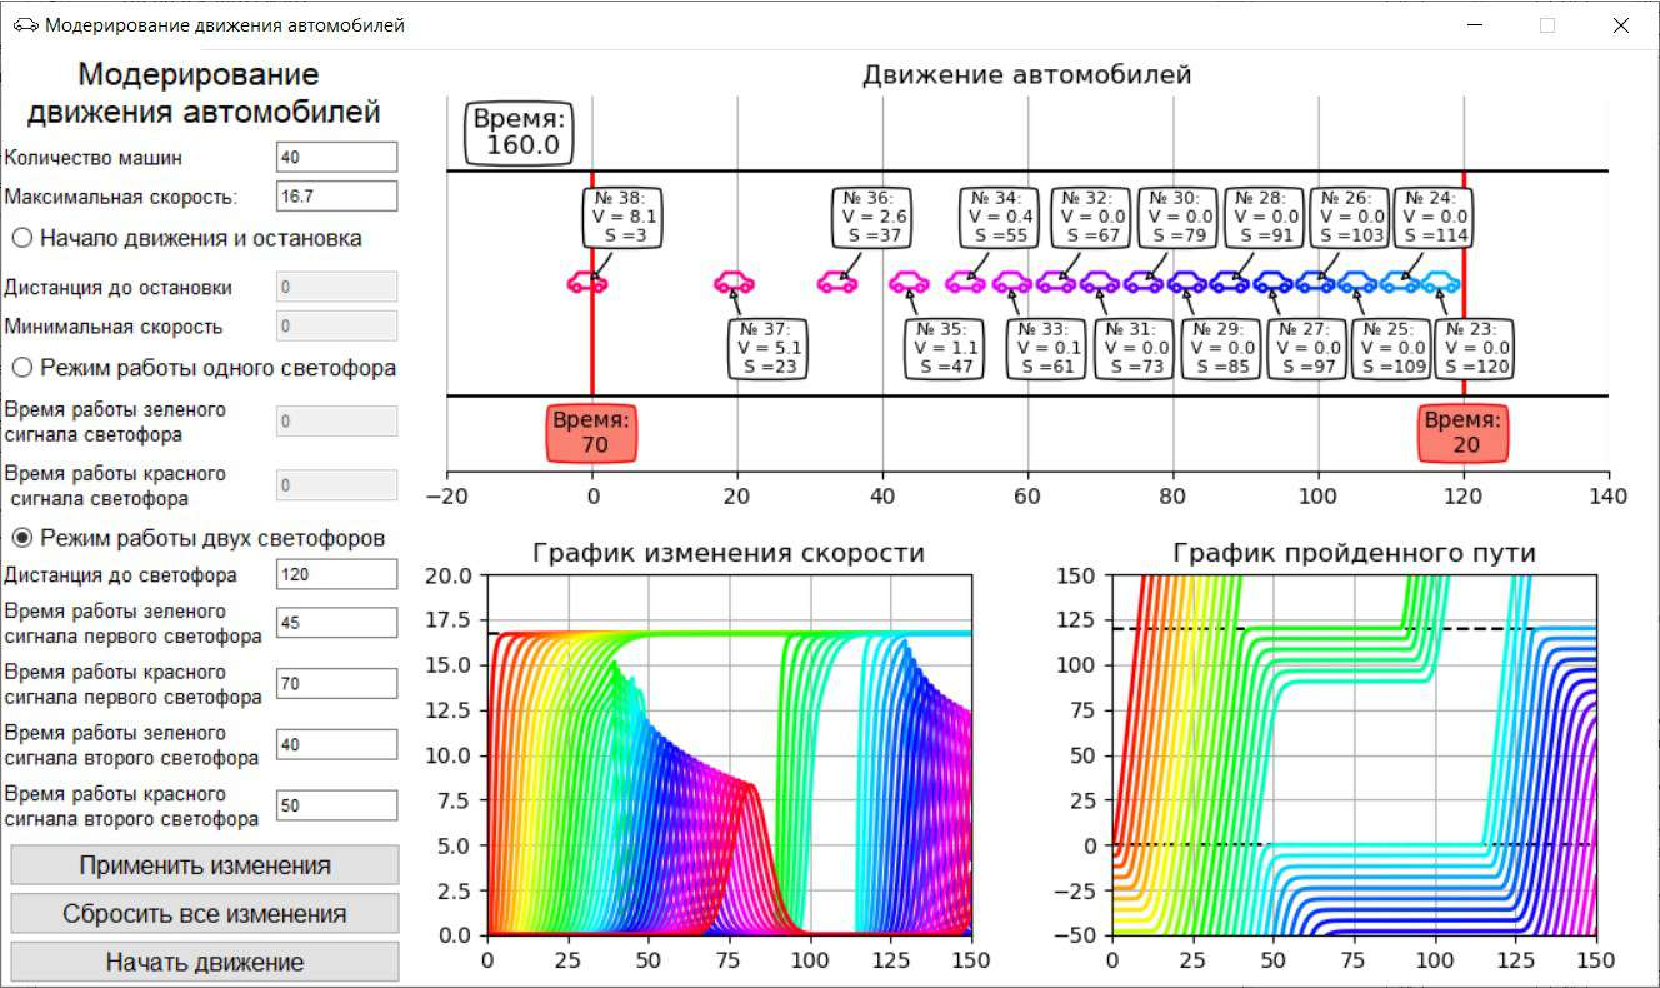
\includegraphics[width=1\linewidth]
			{Images/screens/third_mode_12}
			\caption{Положение автомобилей через 160 секунд после начала движения.}
			\label{third_mode_12}
		\end{minipage}
		\hfill 
		\begin{minipage}[h]{0.48\linewidth}
			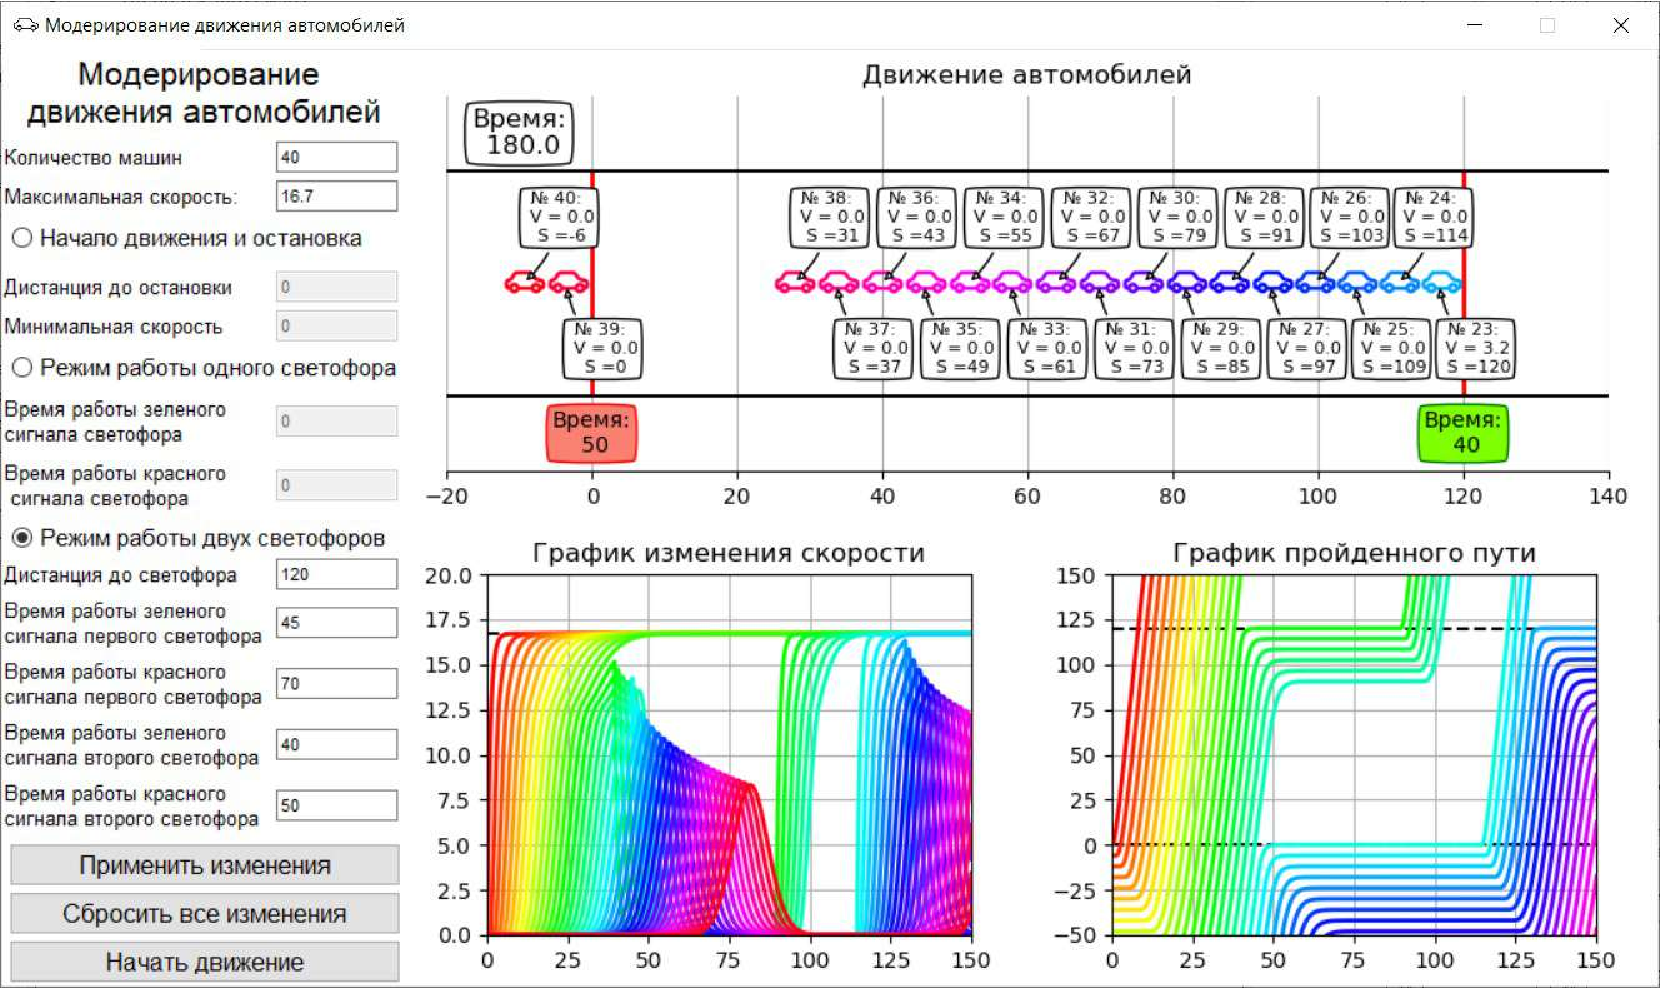
\includegraphics[width=1\linewidth]
			{Images/screens/third_mode_14}
			\caption{Положение автомобилей через 180 секунд после начала движения.}
			\label{third_mode_14}
		\end{minipage}
		\hfill 
		\begin{minipage}[h]{0.48\linewidth}
			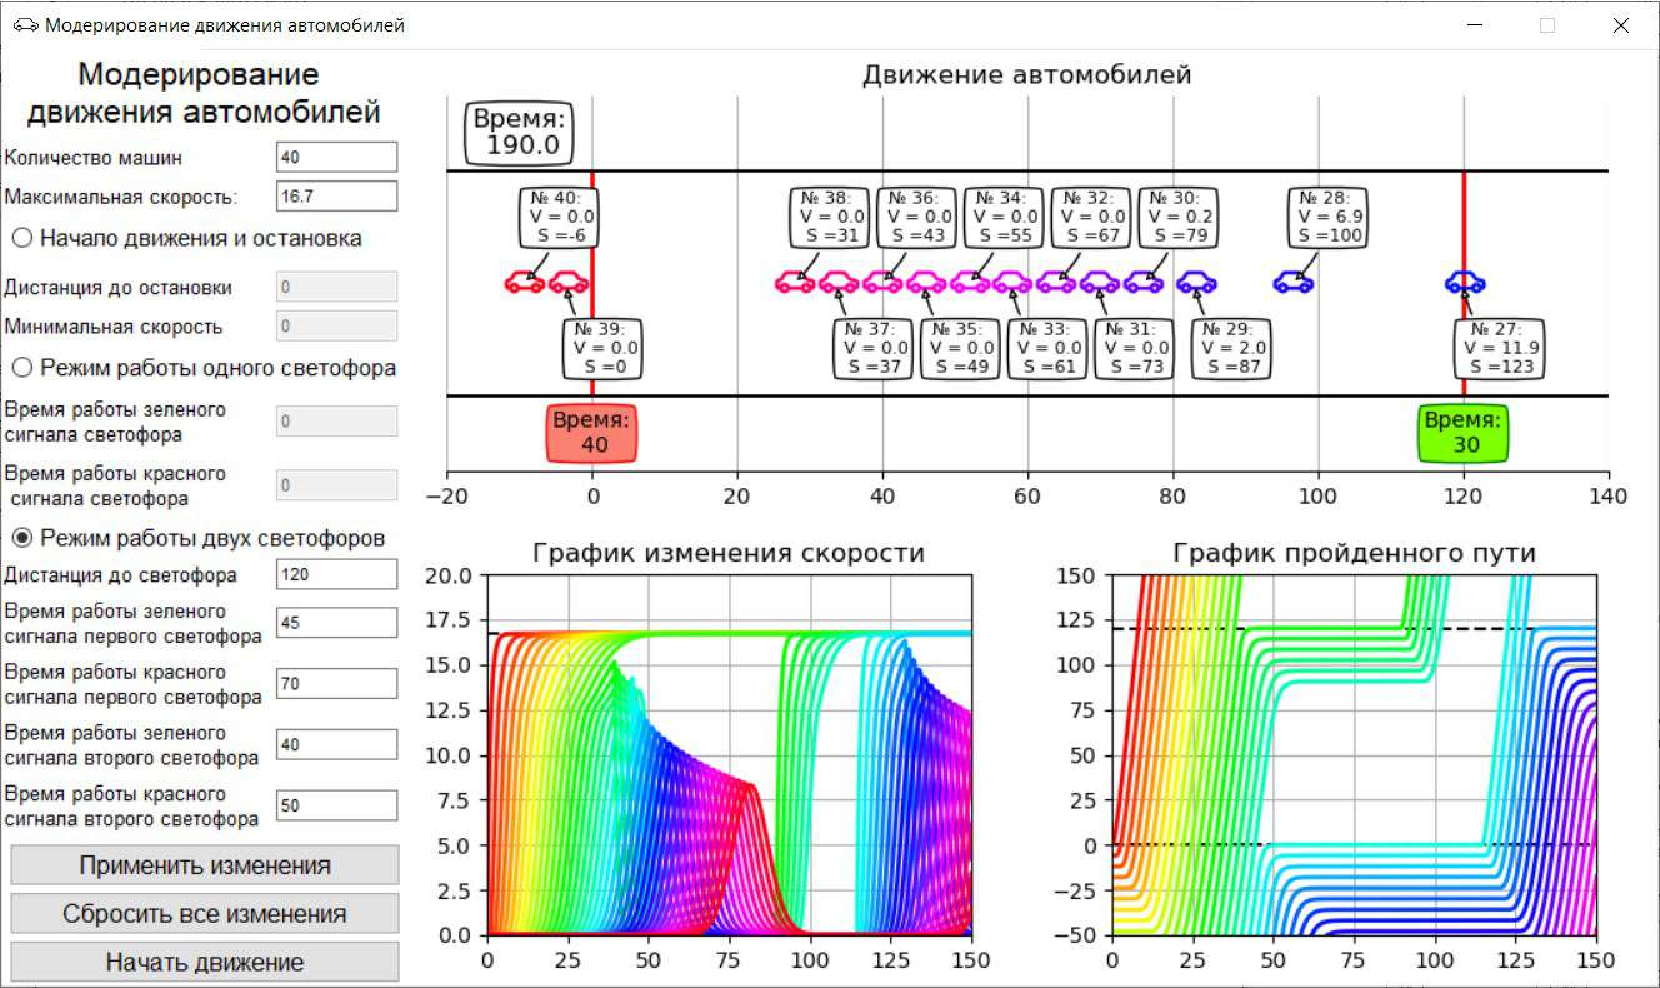
\includegraphics[width=1\linewidth]
			{Images/screens/third_mode_15}
			\caption{Положение автомобилей через 190 секунд после начала движения.}
			\label{third_mode_15}
		\end{minipage}
	\end{center}
\end{figure}

На рисунках \ref{third_mode_1} --- \ref{third_mode_15} показано моделирование нескольких циклов работы двух реальных светофоров. Как видно из рисунков, количество автомобилей, которые проезжают через оба светофора в разработанном приложении равно среднему количеству автомобилей, которые проезжают через оба реальных светофора (приложение \ref{att}). Это ещё раз подтверждает корректность модели \eqref{my_model}, и правильность подобранных параметров (таблица \ref{real_parameters}).

Данный режим работы программы подойдёт для моделирования участков дорог с несколькими идущими друг за другом светофорами. Данный режим программы позволяет отрегулировать режим работы каждого светофора, исключив возникновение заторов и простоев, которые могли бы возникнуть при неудачной настройке реального светофора.  

Таким образом, разработанная программа может упростить настройку светофоров, которая сейчас производится дорожными службами, преимущественно, экспериментальным путём. Экспериментальное регулирование приводит к множеству проблем, так как удачно отрегулировать режим работы светофора с первого раза можно не всегда. Это часто приводит к серьёзным последствиям, таким как пробки и заторы, а в некоторых случаях, и к дорожно транспортным прошествиям. С помощью программы можно заранее смоделировать движение транспортных потоков, посмотреть и изучить их динамику, а затем применить полученные результаты в реальной жизни.

\section*{Заключение}
\addcontentsline{toc}{section}{Заключение}
Исходя из проведённых исследований, можно сделать вывод, что построение математической модели  движения транспортного потока нетривиальная задача и несмотря на значительный прогресс в данной области, полное понимание природы автомобильных проблем ещё не достигнуто. 

В ходе работы была разработана новая математическая модель движения транспортных потоков \eqref{my_model}, которая согласуется с динамикой реального транспортного потока. Это видно из работы программы, которая, используя модель \eqref{my_model}, визуализирует движение автомобилей в потоке. 

Данная работа позволит сделать технологии управления дорожным движением более современными, так как с помощью модели \eqref{my_model} и программы, основанной на ней, можно заранее смоделировать движение транспортного потока, а затем применить полученные результаты в реальной жизни.
\newpage

\begin{thebibliography}{**}
	\addcontentsline{toc}{section}{Список литературы}
	\bibitem{Street}
	Дубелиръ Г.Д. ``Городскiя улицы и мостовыя''. 1912.
	
	\bibitem{TrafficFlow}
	https://spravochnick.ru/logistika/logisticheskie\_potoki/transportnyy\_potok/
	
	\bibitem{probabilistic_model}
	Буслаев А.П., Новиков А.В., Приходько В.М., Таташев А.Г., Яшина М.В. Вероятностные и имитационные подходы к оптимизации автодорожного движения. 2003.
	
	\bibitem{macro_model}
	Куржанский А.А., Куржанский А.Б., Варайя П. Роль макромоделирования в активном управлении транспортной сетью. 2010.
	
	\bibitem{micro_model}
	Зырянов В.В. Применение микромоделирования для прогнозирования развития транспортной инфраструктуры и управления дорожным движение. 2009
	
	\bibitem{GippsModel}
	Wilson R. E. Gipps’ Model of Highway Traffic. 2002.
	
	\bibitem{Shvetsov}
	Швецов В. И. Математическое моделирование транспортных потоков. 2003. 
	
	\bibitem{WolframMathematica}
	https://www.wolfram.com
	
	\bibitem{FirstFollowTheLeaderModel}
	Pipes L.A. An operational analysis of traffic dynamics. 1953. 
		
	\bibitem{RefineFirstFollowTheLeaderModel}
	Chandler R.E., Herman R., Montroll E.W. Traffic dynamics: Studies in car following. 1958.

	\bibitem{GazisModel}
	Gazis D.C., Herman R., Rothery R.W. Nonlinear follow the leader models of traffic flow. 1961.
	
	\bibitem{StudyingGazisModel_1}
	May, Jr. A.D., Kel ler H.E.M. Non-integer car-following models. 1967.
	
	\bibitem{StudyingGazisModel_2}
	K\"{u}hne R.D., R\"{o}diger M.B. Maсrosopiс simulation model for freeway traffic with jams
	and stop-start waves. 1991.
	
	\bibitem{StudyingGazisModel_3}
	K\"{u}hne R.D., Kroen A. Knowledge-based optimization of line сontrol systems for freeways. 1992.

	\bibitem{TreiberModel_1}
	Treiber M., Helbing D. Explanation of observed features of self-organization in traffic flow.
	1999.
	
	\bibitem{TreiberModel_2}
	Treiber M., Hennecke A., Helbing D. Congested traffic states in empirical observations and
	microscopic simulations. 2000.
	
	\bibitem{Heaviside_function}
	Земсков Ю. В. Основы теории сигналов и систем. 2003.
	
	\bibitem{PDD}
	Постановление Правительства РФ от 23.10.1993 N 1090 (ред. от 21.12.2019) ``О Правилах дорожного движения'' (вместе с ``Основными положениями по допуску транспортных средств к эксплуатации и обязанности должностных лиц по обеспечению безопасности дорожного движения'')

	\bibitem{Physics}
	Лазарев Д. А. Совершенствование дорожно-транспортной экспертизы на основе исследования процесса торможения. 2018.

	\bibitem{Python}	
	https://www.python.org
	
	\bibitem{Runge_Kutta}
	Бахвалов Н.С.  Численные методы. 1975. 

\end{thebibliography}

\newpage

\begin{attachment} \label{att}
	\addcontentsline{toc}{section}{Приложение A}
	\begin{center}
		\vspace{1cm}
		\rm{\Large{\textbf{ Наблюдаемые характеристики работы \\ реальных светофоров }}}
		\vspace{\baselineskip}
	\end{center}

\textup{\textbf{Характеристики светофора, расположенного в городе Ярославль на перекрёстке Ленинградского проспекта и улицы Бабича }}
\newline

\noindent\textup{Расстояние до следующего светофора на перекрёстке Ленинградского проспекта и улицы Волгоградской:} 120 метров.

\noindent\textup{Время работы сигналов светофора:}

Время работы зелёного сигнала: 45 секунд.
			
Время работы красного сигнала: 70 секунд.

\noindent\textup{Количество автомобилей, проезжающих через светофор по одной полосе за один цикл работы:}
	
\begin{table}[h!]
	\begin{minipage}{0.23\linewidth}
		
		\centering
		\begin{tabular}{|c|c|}
			\hline
			 & Количество \\ 
			 \raisebox{1.5ex}[0cm]{№}
			 & машин 
			\\\hline
			1 & 21
			\\\hline
			2 & 16
			\\\hline
			3 & 22
			\\\hline
			4 & 18
			\\\hline
			5 & 17
			\\\hline
			6 & 19
			\\\hline
			7 & 22
			\\\hline
			8 & 22
			\\\hline
			9 & 18
			\\\hline
			10 & 16
			\\\hline
		\end{tabular}
	\end{minipage}
	\begin{minipage}{0.23\linewidth}
		\centering
		
		\begin{tabular}{|c|c|}
			\hline
			& Количество \\ 
			\raisebox{1.5ex}[0cm]{№}
			& машин  
			\\\hline
			11 & 16
			\\\hline
			12 & 15
			\\\hline
			13 & 18
			\\\hline
			14 & 21
			\\\hline
			15 & 17
			\\\hline
			16 & 15
			\\\hline
			17 & 16
			\\\hline
			18 & 25
			\\\hline
			19 & 19
			\\\hline
			20 & 18
			\\\hline
		\end{tabular}
	\end{minipage} 
	\begin{minipage}{0.23\linewidth}
		\centering
	
		\begin{tabular}{|c|c|}
			\hline
			& Количество \\ 
			\raisebox{1.5ex}[0cm]{№}
			& машин 
			\\\hline
			21 & 21
			\\\hline
			22 & 20
			\\\hline
			23 & 18
			\\\hline
			24 & 13
			\\\hline
			25 & 15
			\\\hline
			26 & 20
			\\\hline
			27 & 20
			\\\hline
			28 & 22
			\\\hline
			29 & 28
			\\\hline
			30 & 21
			\\\hline
		\end{tabular}
	\end{minipage} 
	\begin{minipage}{0.23\linewidth}
		\centering
	
		\begin{tabular}{|c|c|}
			\hline
			& Количество \\ 
			\raisebox{1.5ex}[0cm]{№}
			& машин 
			\\\hline
			31 & 15
			\\\hline
			32 & 17
			\\\hline
			33 & 19
			\\\hline
			34 & 18
			\\\hline
			35 & 18
			\\\hline
			36 & 14
			\\\hline
			37 & 26
			\\\hline
			38 & 19
			\\\hline
			39 & 20
			\\\hline
			40 & 16
			\\\hline
		\end{tabular}
	\end{minipage}
\end{table}

\noindent Среднее количество автомобилей, проезжающих через светофор: 18.775 $\approx$ 19.
\newline

\noindent\textup{Данные характеристики были собраны в период с 01.03.2020 по 01.05.2020 }.
\newpage

\textup{\textbf{Характеристики светофора, расположенного в городе Ярославль на перекрёстке Ленинградского проспекта и улицы Волгоградской }}
\newline

\noindent\textup{Расстояние до предыдущего светофора на перекрёстке Ленинградского проспекта и улицы Бабича:} 120 метров.

\noindent\textup{Время работы сигналов светофора:}

Время работы зелёного сигнала: 40 секунд.

Время работы красного сигнала: 50 секунд.

\noindent\textup{Количество автомобилей, проезжающих через светофор по одной полосе за один цикл работы:}

\begin{table}[h!]
	\begin{minipage}{0.23\linewidth}
		
		\centering
		\begin{tabular}{|c|c|}
			\hline
			& Количество \\ 
			\raisebox{1.5ex}[0cm]{№}
			& машин 
			\\\hline
			1 & 16
			\\\hline
			2 & 10
			\\\hline
			3 & 15
			\\\hline
			4 & 12
			\\\hline
			5 & 8
			\\\hline
			6 & 11
			\\\hline
			7 & 13
			\\\hline
			8 & 10
			\\\hline
			9 & 12
			\\\hline
			10 & 12
			\\\hline
		\end{tabular}
	\end{minipage}
	\begin{minipage}{0.23\linewidth}
		\centering
		
		\begin{tabular}{|c|c|}
			\hline
			& Количество \\ 
			\raisebox{1.5ex}[0cm]{№}
			& машин  
			\\\hline
			11 & 16
			\\\hline
			12 & 11
			\\\hline
			13 & 15
			\\\hline
			14 & 10
			\\\hline
			15 & 11
			\\\hline
			16 & 13
			\\\hline
			17 & 18
			\\\hline
			18 & 10
			\\\hline
			19 & 10
			\\\hline
			20 & 11
			\\\hline
		\end{tabular}
	\end{minipage} 
	\begin{minipage}{0.23\linewidth}
		\centering
		
		\begin{tabular}{|c|c|}
			\hline
			& Количество \\ 
			\raisebox{1.5ex}[0cm]{№}
			& машин 
			\\\hline
			21 & 9
			\\\hline
			22 & 12
			\\\hline
			23 & 11
			\\\hline
			24 & 13
			\\\hline
			25 & 14
			\\\hline
			26 & 11
			\\\hline
			27 & 10
			\\\hline
			28 & 13
			\\\hline
			29 & 13
			\\\hline
			30 & 13
			\\\hline
		\end{tabular}
	\end{minipage} 
	\begin{minipage}{0.23\linewidth}
		\centering
		
		\begin{tabular}{|c|c|}
			\hline
			& Количество \\ 
			\raisebox{1.5ex}[0cm]{№}
			& машин 
			\\\hline
			31 & 8
			\\\hline
			32 & 10
			\\\hline
			33 & 11
			\\\hline
			34 & 10
			\\\hline
			35 & 12
			\\\hline
			36 & 19
			\\\hline
			37 & 16
			\\\hline
			38 & 14
			\\\hline
			39 & 11
			\\\hline
			40 & 12
			\\\hline
		\end{tabular}
	\end{minipage}
\end{table}
\noindent Среднее количество автомобилей, проезжающих через светофор: 12.15 $\approx$ 12.
\newline

\noindent\textup{Данные характеристики были собраны в период с 01.03.2020 по 01.05.2020 }.
\end{attachment}
\end{document}